%%%%%%%%%%%%%%%%%%%%%%%%%%%%%%%%%%%%%%%%%%%%%%%%%%%%%%%%%%%%%%%%%%%%%%
%% AgriMind -- Elsevier manuscript
%% Build:  pdflatex Manuscript  ->  bibtex Manuscript  ->  pdflatex x2
%%%%%%%%%%%%%%%%%%%%%%%%%%%%%%%%%%%%%%%%%%%%%%%%%%%%%%%%%%%%%%%%%%%%%%
\documentclass[preprint,12pt]{elsarticle}
\usepackage[left=2cm, right=2cm, top=2cm, bottom=2cm]{geometry}

\usepackage{amssymb}
\usepackage{amsmath}
\usepackage{algorithmic}
\usepackage{algorithm}
\usepackage{booktabs}
\usepackage{multirow}
\usepackage{graphicx}
\usepackage{pifont}
\usepackage{stfloats}
\usepackage[caption=false,font=normalsize,labelfont=sf,textfont=sf]{subfig}
\usepackage{balance}
\usepackage{bm}
\usepackage{url}

%% Float placement: LaTeX's defaults are conservative enough that a
%% table-heavy manuscript pushes most floats to the end. These relax the
%% per-page limits so tables and figures settle near the text that
%% discusses them.
\setcounter{topnumber}{3}
\setcounter{bottomnumber}{2}
\setcounter{totalnumber}{5}
\renewcommand{\topfraction}{0.9}
\renewcommand{\bottomfraction}{0.7}
\renewcommand{\textfraction}{0.1}
\renewcommand{\floatpagefraction}{0.75}

\begin{document}

\begin{frontmatter}

\title{Governed Multi-Agent Reasoning for Agricultural Decision Support:
A Bayesian Trust Layer with Reproducible Reliability Evaluation}

\author[label1]{Author One\corref{cor1}}
\author[label1]{Author Two}
\author[label1]{Author Three}

\affiliation[label1]{organization={Department of Computer Science and Engineering,
Amrita School of Computing, Amrita Vishwa Vidyapeetham},
addressline={},
city={Coimbatore},
postcode={641112},
state={Tamil Nadu},
country={India}}

\cortext[cor1]{Corresponding author. Email: author.one@example.edu}

\begin{abstract}
Farm advisory systems built on large language models rarely state how far
their own components can be trusted, and are seldom evaluated for what
happens when a data source or model provider fails mid-decision. This work
presents AgriMind, a ten-stage multi-agent advisory pipeline in which five
heterogeneous specialists---weather, soil, satellite, market and
historical---are routed dynamically by intent and by live data
availability, fused through a collaborative reasoning stage, and wrapped by
a Beta--Bernoulli trust layer that gates each agent before execution and
updates its posterior afterwards. Every language-model stage carries a
deterministic fallback, so provider failure degrades output quality rather
than terminating the request. A reproducible benchmark of controlled
single-variable perturbations, replayed against fixed fixtures, measures
routing, rule-consistency, detection, calibration and latency behaviour.
Across eleven scenarios no task failures and no routing errors were
observed, rule-consistency reached 63.6\% overall and 70.0\% excluding
scenarios that deliberately probe a documented gap in the decision
vocabulary; two grounding instruments with no generative model in the loop
returned no findings. Concurrent execution cut end-to-end latency by
23.6\%, though the resulting 426.6\,s remains far too slow for field
use. The sample is small and ground truth is
rule-derived rather than agronomist-validated, so these figures
characterise mechanism rather than field performance.
\end{abstract}

\begin{keyword}
Multi-agent systems \sep Large language models \sep Precision agriculture
\sep Bayesian trust modelling \sep AI governance \sep Explainable decision support
\end{keyword}

\end{frontmatter}

%%%%%%%%%%%%%%%%%%%%%%%%%%%%%%%%%%%%%%%%%%%%%%%%%%%%%%%%%%%%%%%%%%%%%%
\section{Introduction}
\label{sec:intro}

Smallholder farming decisions are rarely bounded by a single discipline. A
grower asking whether to irrigate is simultaneously asking a question about
canopy water stress, about soil moisture retention, about the rainfall
forecast, and---if the crop is near maturity---about whether the harvest is
worth more next week than this one. Precision agriculture has produced
strong models for each of these questions in isolation, but the task of
combining them into one defensible recommendation remains largely open.

Recent work has begun to address this by assigning distinct models to
distinct sub-problems and coordinating them as agents. Zuzu\'arregui et
al.~\cite{zuzuarregui2025oneforall} apply an LLM controller to farm robotic
task execution; Tariq et al.~\cite{tariq2025edge} feed supervised vision and
weather classifiers into a rule-based decision layer at the edge; Kandamali
et al.~\cite{kandamali2025cottonbot} build a retrieval-augmented cotton
advisor whose agentic tools pull live soil-moisture and weather data. Murad
et al.~\cite{murad2026agentic} coordinate four agents (soil, weather,
disease vision, supervisor) for smart farming, and Davcev et
al.~\cite{davcev2026multiagent} formalise the same coordination problem as a
multi-agent partially observable Markov decision process. The direction is
well motivated and the reported component accuracies are high.

What this literature does not yet establish is how such a system behaves
when it is wrong, uncertain, or partially blind. Three gaps recur. First,
agent selection is typically static: the same specialists run for every
query, regardless of whether the question needs them or whether their data
source has anything to report. Second, the systems have no internal notion
of how much a given agent should be believed---an agent that has failed
repeatedly is trusted exactly as much as one that has never failed. Raza et
al.~\cite{raza2025trism} argue this specific point for agentic AI at large,
and Gavai and Heringa~\cite{gavai2025agentic} frame it as a governance
requirement, but neither instantiates a measured mechanism. Third, and most
consequentially for deployment, evaluation is almost always conducted under
conditions where every component works. Reported figures therefore describe
the best case, and say little about the far more common situation in which
a satellite tile is cloud-covered, an API is rate-limited, or a provider
quota is exhausted.

This paper addresses those three gaps together. We present AgriMind, a
multi-agent agricultural advisory pipeline whose distinguishing property is
not the number of agents it runs but the fact that it maintains, updates,
and acts upon an explicit belief about each agent's reliability, and that
its evaluation is designed to measure behaviour under degradation rather
than to avoid it. We are explicit throughout that this evaluation is a
controlled synthetic perturbation suite---a systems-level test harness,
not a field trial---and Section~\ref{sec:limitations} states what that
does and does not license us to claim.

\subsection*{Contributions}

\begin{enumerate}
\item \textbf{Availability-aware dynamic routing.} A planner that selects
specialists jointly on query intent \emph{and} on whether each source
actually holds usable data, rather than on a fixed intent-to-agent map.
No routing errors were observed on the ten benchmark scenarios, nor on
eight held-out queries using crops and phrasings absent from prompt
development (Section~\ref{sec:results}). We report these as observed
counts; the sample does not support a rate estimate.

\item \textbf{An operative trust layer, and its measured calibration.}
The underlying estimator is a standard Beta--Bernoulli conjugate update
and we claim no mathematical novelty in it. The contribution is
system-level: the posterior is wired into the execution path as a
pre-execution gate rather than kept as an audit annotation, and its
calibration against observed reliability is measured and reported
(mean absolute error 0.228) rather than assumed. To our knowledge no
prior agricultural multi-agent system reports trust calibration at
all.

\item \textbf{Fallback-complete degradation, plus an LLM-free grounding
check.} Every language-model stage has a deterministic counterpart, and no
run failed to return a complete recommendation---including runs in which a
provider failed mid-request. Because three metrics rely on an LLM judge, we
additionally introduce two grounding instruments with no generative model
in the loop: a deterministic numeric check verifying every
measurement-cued quantity against the raw context, and an entailment
classifier testing each generated assertion against context premises for
contradiction (Section~\ref{sec:grounding}). Both return zero findings,
corroborating the LLM-judged result on the axes they cover.

\item \textbf{A reproducible perturbation benchmark with rule-derived ground
truth.} Scenarios are built by cloning genuine collected contexts,
neutralising them, and applying exactly one perturbation that crosses a
threshold already present in the crop's own agronomic profile---making
ground truth auditable and every run replayable.

\item \textbf{Concurrency-consistent ablation.} Specialists execute
concurrently, cutting mean end-to-end latency by 23.6\%; critically, the
ablation baselines were made to use the same concurrency, so the reported
latency differences reflect architecture rather than execution strategy
(Section~\ref{sec:ablation}).
\end{enumerate}

The remainder of the paper is organised as follows.
Section~\ref{sec:related} reviews recent multi-agent, governance and
explainability work and identifies the specific gap addressed here.
Section~\ref{sec:dataset} describes the data sources and benchmark
construction. Section~\ref{sec:proposed} details the architecture and its
formal treatment. Section~\ref{sec:ablation} reports the ablation study,
Section~\ref{sec:results} the main results, and
Section~\ref{sec:comparison} positions them against prior systems.
Section~\ref{sec:conclusion} concludes.

%%%%%%%%%%%%%%%%%%%%%%%%%%%%%%%%%%%%%%%%%%%%%%%%%%%%%%%%%%%%%%%%%%%%%%
\section{Literature Review}
\label{sec:related}

\subsection{Multi-agent architectures for agriculture}

The closest architectural precedent is Murad et
al.~\cite{murad2026agentic}, whose four-agent framework (soil, weather,
disease vision, supervisor) is structurally a subset of the design proposed
here. They report strong per-agent figures---96\% validation accuracy for
soil classification via a 1D-CNN, 0.27 MAE for weather regression via a
GRU, and 98.5\% validation accuracy for disease vision via MobileViT---but
the supervisor performs orchestration only; there is no representation of
agent trustworthiness and no reported behaviour under component failure.
Davcev et al.~\cite{davcev2026multiagent} approach the same coordination
problem theoretically, formalising it as an MPOMDP, and report YOLO26
mAP50 of 72--77\% alongside 96.5\% TabPFN accuracy; the authors themselves
present this as a feasibility demonstration rather than a validated
deployment. Srinivasu et al.~\cite{srinivasu2026federated} combine agentic
AI with federated learning for disease and weed detection (96.4\%
classification accuracy, mAP@0.5 up to 0.978) but state explicitly that
true multi-agent decision logic is deferred to future work---which is
precisely the collaborative reasoning and executive arbitration stage this
paper contributes.

\subsection{LLM agents and retrieval-augmented advisory systems}

CottonBot~\cite{kandamali2025cottonbot} is the nearest LLM-agent analogue:
a RAG advisor with agentic tools reaching live soil-moisture and weather
data. Its benchmarking is rigorous where ground truth exists---MRR 0.886
and Recall@5 0.948 for retrieval, faithfulness 0.968 at 6.2\,s per query
for generation, and an irrigation forecast MAE below 1.0 against a manual
baseline of 1.4. That rigour is instructive, and also illustrates the
boundary condition: it is achievable because sensor logs supply an external
ground truth, which a general advisory recommendation does not have. Sawant
et al.~\cite{sawant2026llm} contribute the most complete generation-quality
metric taxonomy we found, spanning Precision@K, MRR and NDCG for retrieval
and BLEU, ROUGE and BERTScore with a manual claim-level faithfulness audit
for generation. AgroAskAI~\cite{cantonjos2026agroaskai} is architecturally
closest on governance: its Reviewer agent catches hallucinations and
triggers regeneration, filling the same functional role as the trust gate
proposed here, though its evaluation is qualitative---counted mentions
across 20 queries against ChatGPT and CROPWAT---rather than a quantitative
reliability measurement.

\subsection{Trust, governance and Bayesian modelling}

Liu~\cite{liu2020beta} provides the theoretical basis for the trust
posterior used here, formalising a Beta-distribution trust model with the
conjugate update this work implements, and documenting two extensions we do
not yet adopt: a forgetting factor for recency weighting, and third-party
trust aggregation. Raza et al.~\cite{raza2025trism} propose TRiSM for
agentic AI and supply the trustworthiness framing we adapt, together with a
component synergy score aimed specifically at coordination quality. Gavai
and Heringa~\cite{gavai2025agentic} organise governance around
transparency, fairness, sustainability and human oversight, but at a
discursive level; the trust layer and decision trace reported here are a
concrete, measured instantiation of that framing. From an adjacent domain,
UA-Fusion~\cite{shao2025uafusion} is the most rigorously benchmarked
uncertainty-aware fusion system reviewed (71.2\% mAP on nuScenes, with
ablation-isolated gains attributable to explicit uncertainty modelling),
and supports the principle of propagating rather than suppressing
component-level uncertainty.

\subsection{Explainability}

AgroXAI~\cite{turgut2024agroxai} and the decision-support system of Swati
et al.~\cite{swati2026dss} both apply post-hoc SHAP and LIME explanations
over classical classifiers, reporting accuracies in the 89--99\% band
(AgroXAI approximately 99.2\% with Random Forest; Swati et al.\ 92.9\% for
soil CNN, 92.4\% for crop recommendation, 94.7\% for fertiliser XGBoost).
These figures anchor the accuracy range achievable on the individual
sub-tasks, and also mark why a direct numerical comparison with the present
work would be misleading: those systems classify a single labelled target,
whereas the pipeline evaluated here arbitrates among four active,
partially conflicting evidence streams with no single label to score against. The
reviews of Pai et al.~\cite{pai2025review} and Saki et
al.~\cite{saki2024fusion} catalogue the field; the latter's finding that
transformer-based fusion remains a minority (11\% of 1{,}201 surveyed
papers) situates LLM-based integration as an actively developing rather
than settled approach.

\subsection{Identified gap}

Table~\ref{tab:litreview} summarises the reviewed work. Across it, the
dominant evaluation pattern is supervised accuracy on a narrow labelled
sub-task, measured under nominal conditions. Three properties are
consistently absent: routing that accounts for data availability, an
operative (not merely descriptive) trust mechanism, and any measurement of
behaviour when components fail. This paper targets that intersection.

\begin{table}[htbp]
\centering
\caption{Summary of reviewed literature and its relation to the present work.}
\label{tab:litreview}
\footnotesize
\begin{tabular}{@{}p{0.55cm}p{2.9cm}p{3.0cm}p{3.35cm}p{3.5cm}@{}}
\toprule
\textbf{Ref} & \textbf{Title / focus} & \textbf{Methodology} & \textbf{Reported contribution} & \textbf{Limitation w.r.t.\ this work} \\
\midrule
\cite{murad2026agentic} & Agentic AI for traditional farming & 4 agents; 1D-CNN, GRU, MobileViT & Soil 96\% val.\ acc.; weather 0.27 MAE; disease 98.5\% & Supervisor orchestrates only; no trust model, no failure-mode evaluation \\
\cite{davcev2026multiagent} & Multi-agent precision agriculture & MPOMDP formalisation; YOLO26, TabPFN & mAP50 72--77\%; 96.5\% accuracy & Authors state it is a feasibility demo, not validated deployment \\
\cite{srinivasu2026federated} & Agentic AI + federated learning & Federated CNN for disease/weed & 96.4\% acc.; mAP@0.5 0.978 & Multi-agent decision logic explicitly left to future work \\
\cite{kandamali2025cottonbot} & CottonBot RAG advisor & RAG + agentic tools, Llama 3.1 8B & MRR 0.886; faithfulness 0.968; 6.2\,s/query & Single crop; ground truth from sensors only; no governance layer \\
\cite{sawant2026llm} & LLM advisory metric taxonomy & Retrieval + generation metrics & Precision@K, NDCG, BERTScore, faithfulness audit & Metric framework rather than a deployed multi-agent system \\
\cite{cantonjos2026agroaskai} & AgroAskAI & Reviewer agent catches hallucination & 16/20 institutional-support mentions vs.\ 4/20, 0/20 & Qualitative counts over 20 queries; no reliability quantification \\
\cite{zuzuarregui2025oneforall} & One For All & LLM control of farm robots & 7/10 robot missions succeeded & Task execution, not advisory decision-making \\
\cite{tariq2025edge} & Edge agentic framework & Vision + weather classifiers, rule layer & 88\% and 93\% classification accuracy & Decision layer is rule-based, not LLM-reasoned; no trust model \\
\cite{liu2020beta} & Beta-distribution trust model & Bayesian conjugate updating & Formal BDTM with forgetting factor & Theory only; not instantiated in an agricultural pipeline \\
\cite{raza2025trism} & TRiSM for agentic AI & Governance framework, synergy scores & Trust/risk/security taxonomy & Framework proposal; no measured deployment \\
\cite{gavai2025agentic} & Agentic AI governance review & Ethical quartet framing & Transparency, fairness, oversight & Discursive; no concrete mechanism or metric \\
\cite{shao2025uafusion} & UA-Fusion & Aleatoric/epistemic uncertainty fusion & 71.2\% mAP on nuScenes & Autonomous driving domain; not agricultural \\
\cite{turgut2024agroxai} & AgroXAI & SHAP/LIME over RF and DT & $\approx$99.2\% accuracy & Post-hoc explanation of one classifier; no multi-agent arbitration \\
\cite{swati2026dss} & Crop/fertiliser DSS & CNN, RF, XGBoost + XAI & 92.9\%, 92.4\%, 94.7\% & Independent classifiers; no cross-source conflict handling \\
\cite{saki2024fusion} & Remote-sensing fusion review & Bibliometric survey (1{,}201 papers) & Transformer fusion at 11\% share & Survey; no original system or metrics \\
\cite{pai2025review} & Precision agriculture review & Literature survey & Field synthesis & Survey; no original system or metrics \\
\bottomrule
\end{tabular}
\end{table}

%%%%%%%%%%%%%%%%%%%%%%%%%%%%%%%%%%%%%%%%%%%%%%%%%%%%%%%%%%%%%%%%%%%%%%
\section{Dataset Description}
\label{sec:dataset}

\subsection{Operational data sources}

The pipeline draws on five heterogeneous streams, four of which are live
external services. Table~\ref{tab:sources} lists them with the fields each
contributes.

\begin{table}[htbp]
\centering
\caption{Operational data sources and the fields each contributes.}
\label{tab:sources}
\footnotesize
\begin{tabular}{@{}p{1.8cm}p{3.6cm}p{1.6cm}p{7.4cm}@{}}
\toprule
\textbf{Stream} & \textbf{Source} & \textbf{Access} & \textbf{Fields consumed} \\
\midrule
Weather & Open-Meteo forecast API & Live REST & temperature\_2m, relative\_humidity\_2m, rain, wind\_speed\_10m, surface\_pressure \\
Soil & ISRIC SoilGrids v2.0 & Live REST & phh2o, nitrogen, soc, sand, clay, silt, cec, bdod (0--5\,cm, mean) \\
Satellite & Sentinel-2 via Google Earth Engine & Live, cloud-masked & NDVI, EVI, SAVI, NDWI, soil exposure, cloud cover, acquisition date \\
Market & Agmarknet via data.gov.in & Live REST & state, district, market, commodity, min/max/modal price, arrival date \\
Historical & Local SQLite (\texttt{farm\_history}) & Local & last five records per crop; empty history treated as a valid signal \\
\bottomrule
\end{tabular}
\end{table}

Soil and market streams each retain a curated local table as a fallback,
used when the live service has no coverage for a coordinate or is
unreachable. This matters in practice: SoilGrids masks built-up land, so a
query centred on a city returns no soil profile at all. Treating that as a
legitimate ``no data'' answer rather than an error is what allows the
routing layer described in Section~\ref{sec:proposed} to exclude an agent
that has nothing to analyse. The schemas of the two fallback tables are
given in Table~\ref{tab:schema}.

\begin{table}[htbp]
\centering
\caption{Schema of the local fallback tables. Both cover 30 districts of
Tamil Nadu, India.}
\label{tab:schema}
\footnotesize
\begin{tabular}{@{}p{2.4cm}p{1.4cm}p{11.0cm}@{}}
\toprule
\textbf{Table} & \textbf{Records} & \textbf{Columns} \\
\midrule
\texttt{soil\_data} & 150 & State, District, Latitude, Longitude, Texture, pH, Nitrogen, Organic\_Carbon, Sand, Clay, Silt, CEC, Bulk\_Density, Field\_Capacity, Wilting\_Point, Drainage \\
\texttt{market\_prices} & 450 & State, District, Latitude, Longitude, Crop, Market, Min\_Price, Max\_Price, Modal\_Price, Trend, Last\_Updated \\
\bottomrule
\end{tabular}
\end{table}

The market table spans 90 markets across 30 districts and 15 commodities
(rice, cotton, maize, groundnut, sugarcane, banana, mango, tomato, onion,
chilli, turmeric, coconut, tapioca, black gram and gingelly). Because
Agmarknet publishes prices without geometry, market coordinates are joined
from this local reference table even when prices are live; a live record
whose market cannot be geo-located is discarded rather than assigned
approximate coordinates, since the ranking function scores partly on
distance.

Agmarknet also publishes no trend field, and a single day's snapshot
carries no trend information. Rather than infer one, the system persists
each observed modal price and derives the trend by comparison with the
previous observation for that market--commodity pair, reporting
\texttt{Unknown} on first sighting. A change of magnitude below 2\% is
reported as \texttt{Stable}, since day-to-day mandi fluctuation of a few
percent is not a trend.

\subsection{Evaluation benchmark}

Measuring a recommendation pipeline is complicated by the absence of a
single correct answer. We therefore construct a controlled benchmark by
perturbation, following the procedure in
Fig.~\ref{fig:benchmark}. A genuine context previously collected by the
system---real Open-Meteo readings, real Sentinel-2 indices---is cloned and
neutralised, resetting every field to a mid-optimal value for that crop.
Exactly one field is then perturbed so that it unambiguously crosses a
threshold already present in that crop's own agronomic profile: soil pH is
driven 2.3 units below the crop's stated minimum, NDWI below its
high-stress threshold, NDVI below its poor threshold, and so on. The
ground-truth decision is whatever that crossed threshold implies.

\begin{figure}[htbp]
\centering
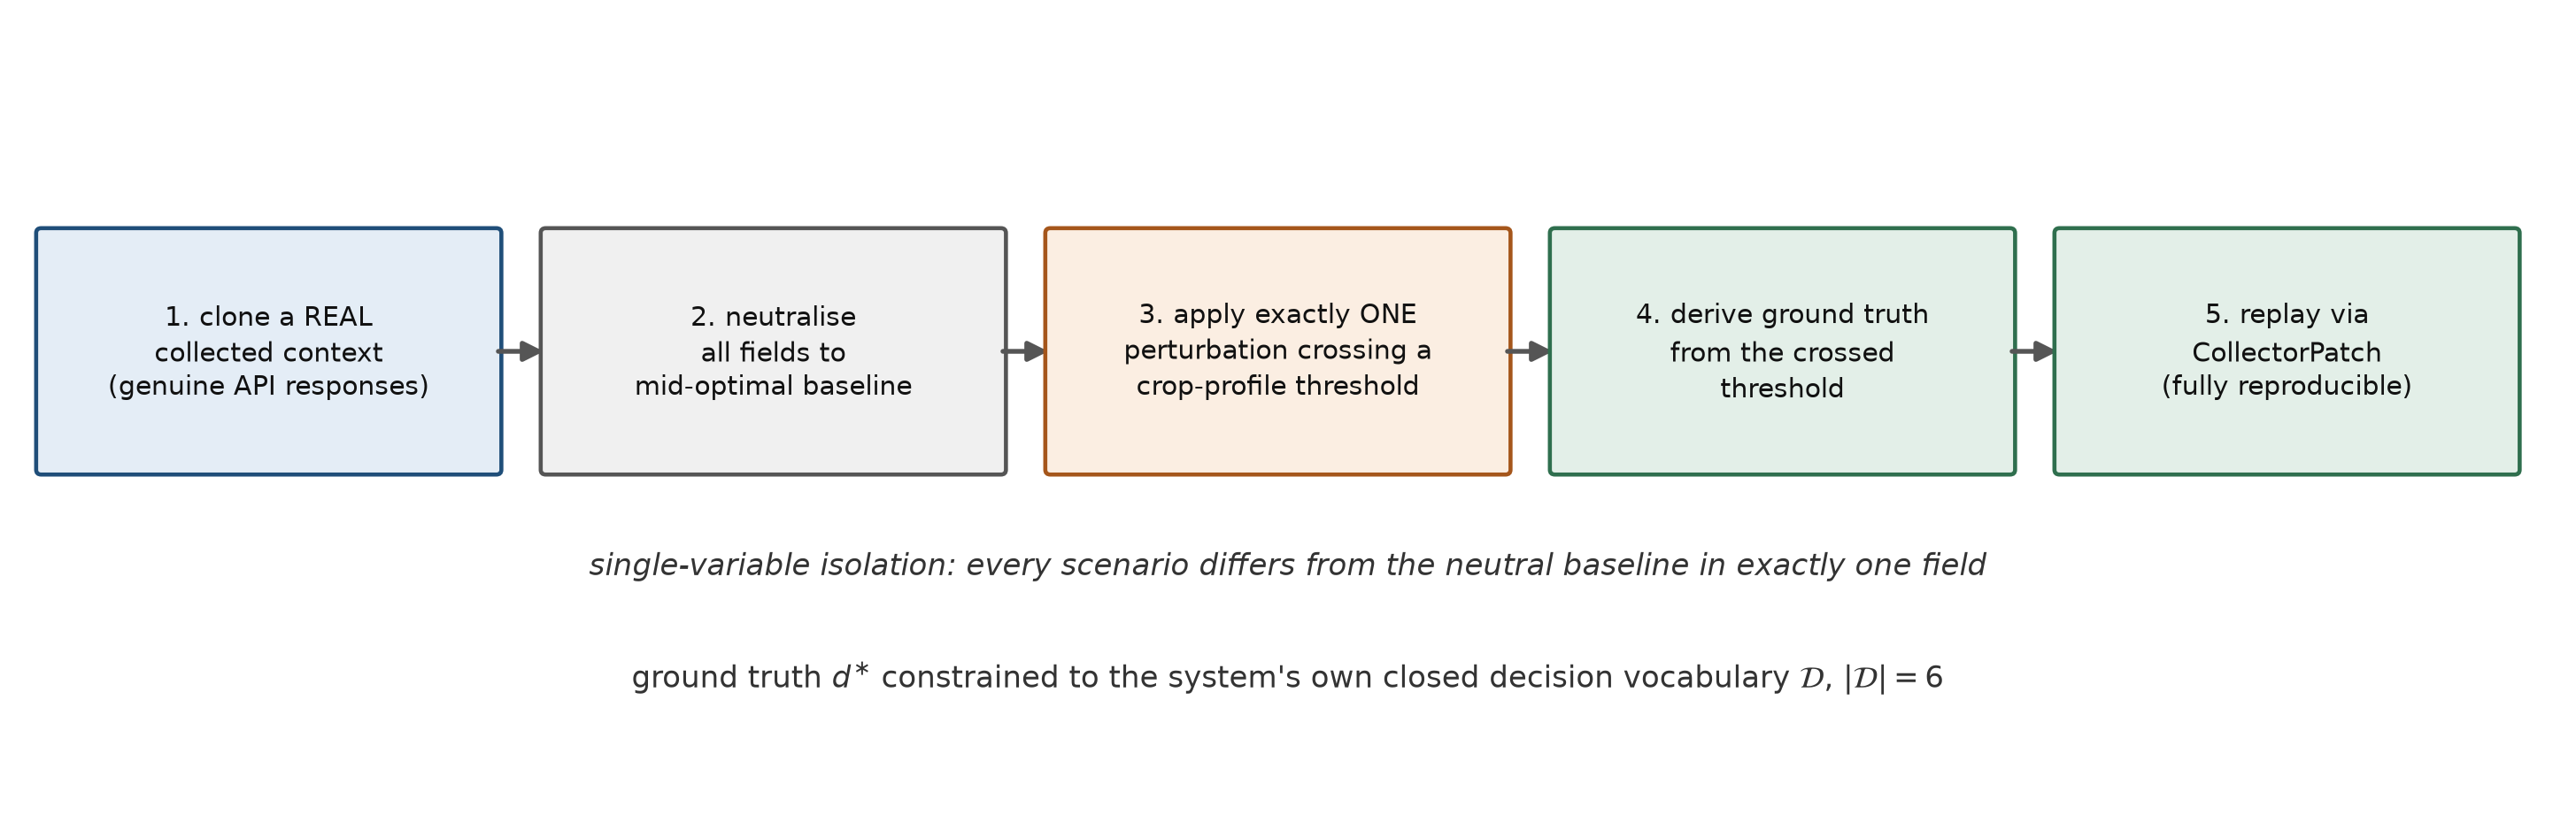
\includegraphics[width=0.95\textwidth]{figures/fig_benchmark_construction.png}
\caption{Benchmark construction. Cloning a real context and perturbing a
single field isolates one variable per scenario while keeping every run
byte-for-byte replayable.}
\label{fig:benchmark}
\end{figure}

Two properties follow. First, single-variable isolation: each scenario
differs from the neutral baseline in exactly one field, so an incorrect
decision is attributable. Second, replayability: fixtures are injected in
place of live collectors, so a run is reproducible independently of what
the live APIs return on a given day.

Ground-truth decisions are necessarily drawn from the system's own closed
decision vocabulary $\mathcal{D}$, $|\mathcal{D}|=6$: \{Immediate
Irrigation, Field Inspection, Apply Nitrogen Fertilizer, Apply Organic
Manure, Prepare for Harvest and Selling, Continue Monitoring\}. We state
this plainly because it bounds the interpretation of the rule-consistency rate, and
we return to it in Section~\ref{sec:limitations}.

%%%%%%%%%%%%%%%%%%%%%%%%%%%%%%%%%%%%%%%%%%%%%%%%%%%%%%%%%%%%%%%%%%%%%%
\section{Proposed Work}
\label{sec:proposed}

\subsection{Overview and notation}

Let $A=\{a_1,\dots,a_5\}$ denote the specialist set (weather, soil,
satellite, market, historical), $q$ a natural-language query, $c$ a crop,
and $\ell=(\phi,\lambda)$ a location. A request is the triple $(q,c,\ell)$.
The pipeline proceeds in ten stages, shown in
Fig.~\ref{fig:architecture}, and is best read as three concerns: acquiring
and normalising evidence (Stages 1--3), deciding what to reason over and
doing so (Stages 4--8), and accounting for the result (Stages 9--10).

\begin{figure}[htbp]
\centering
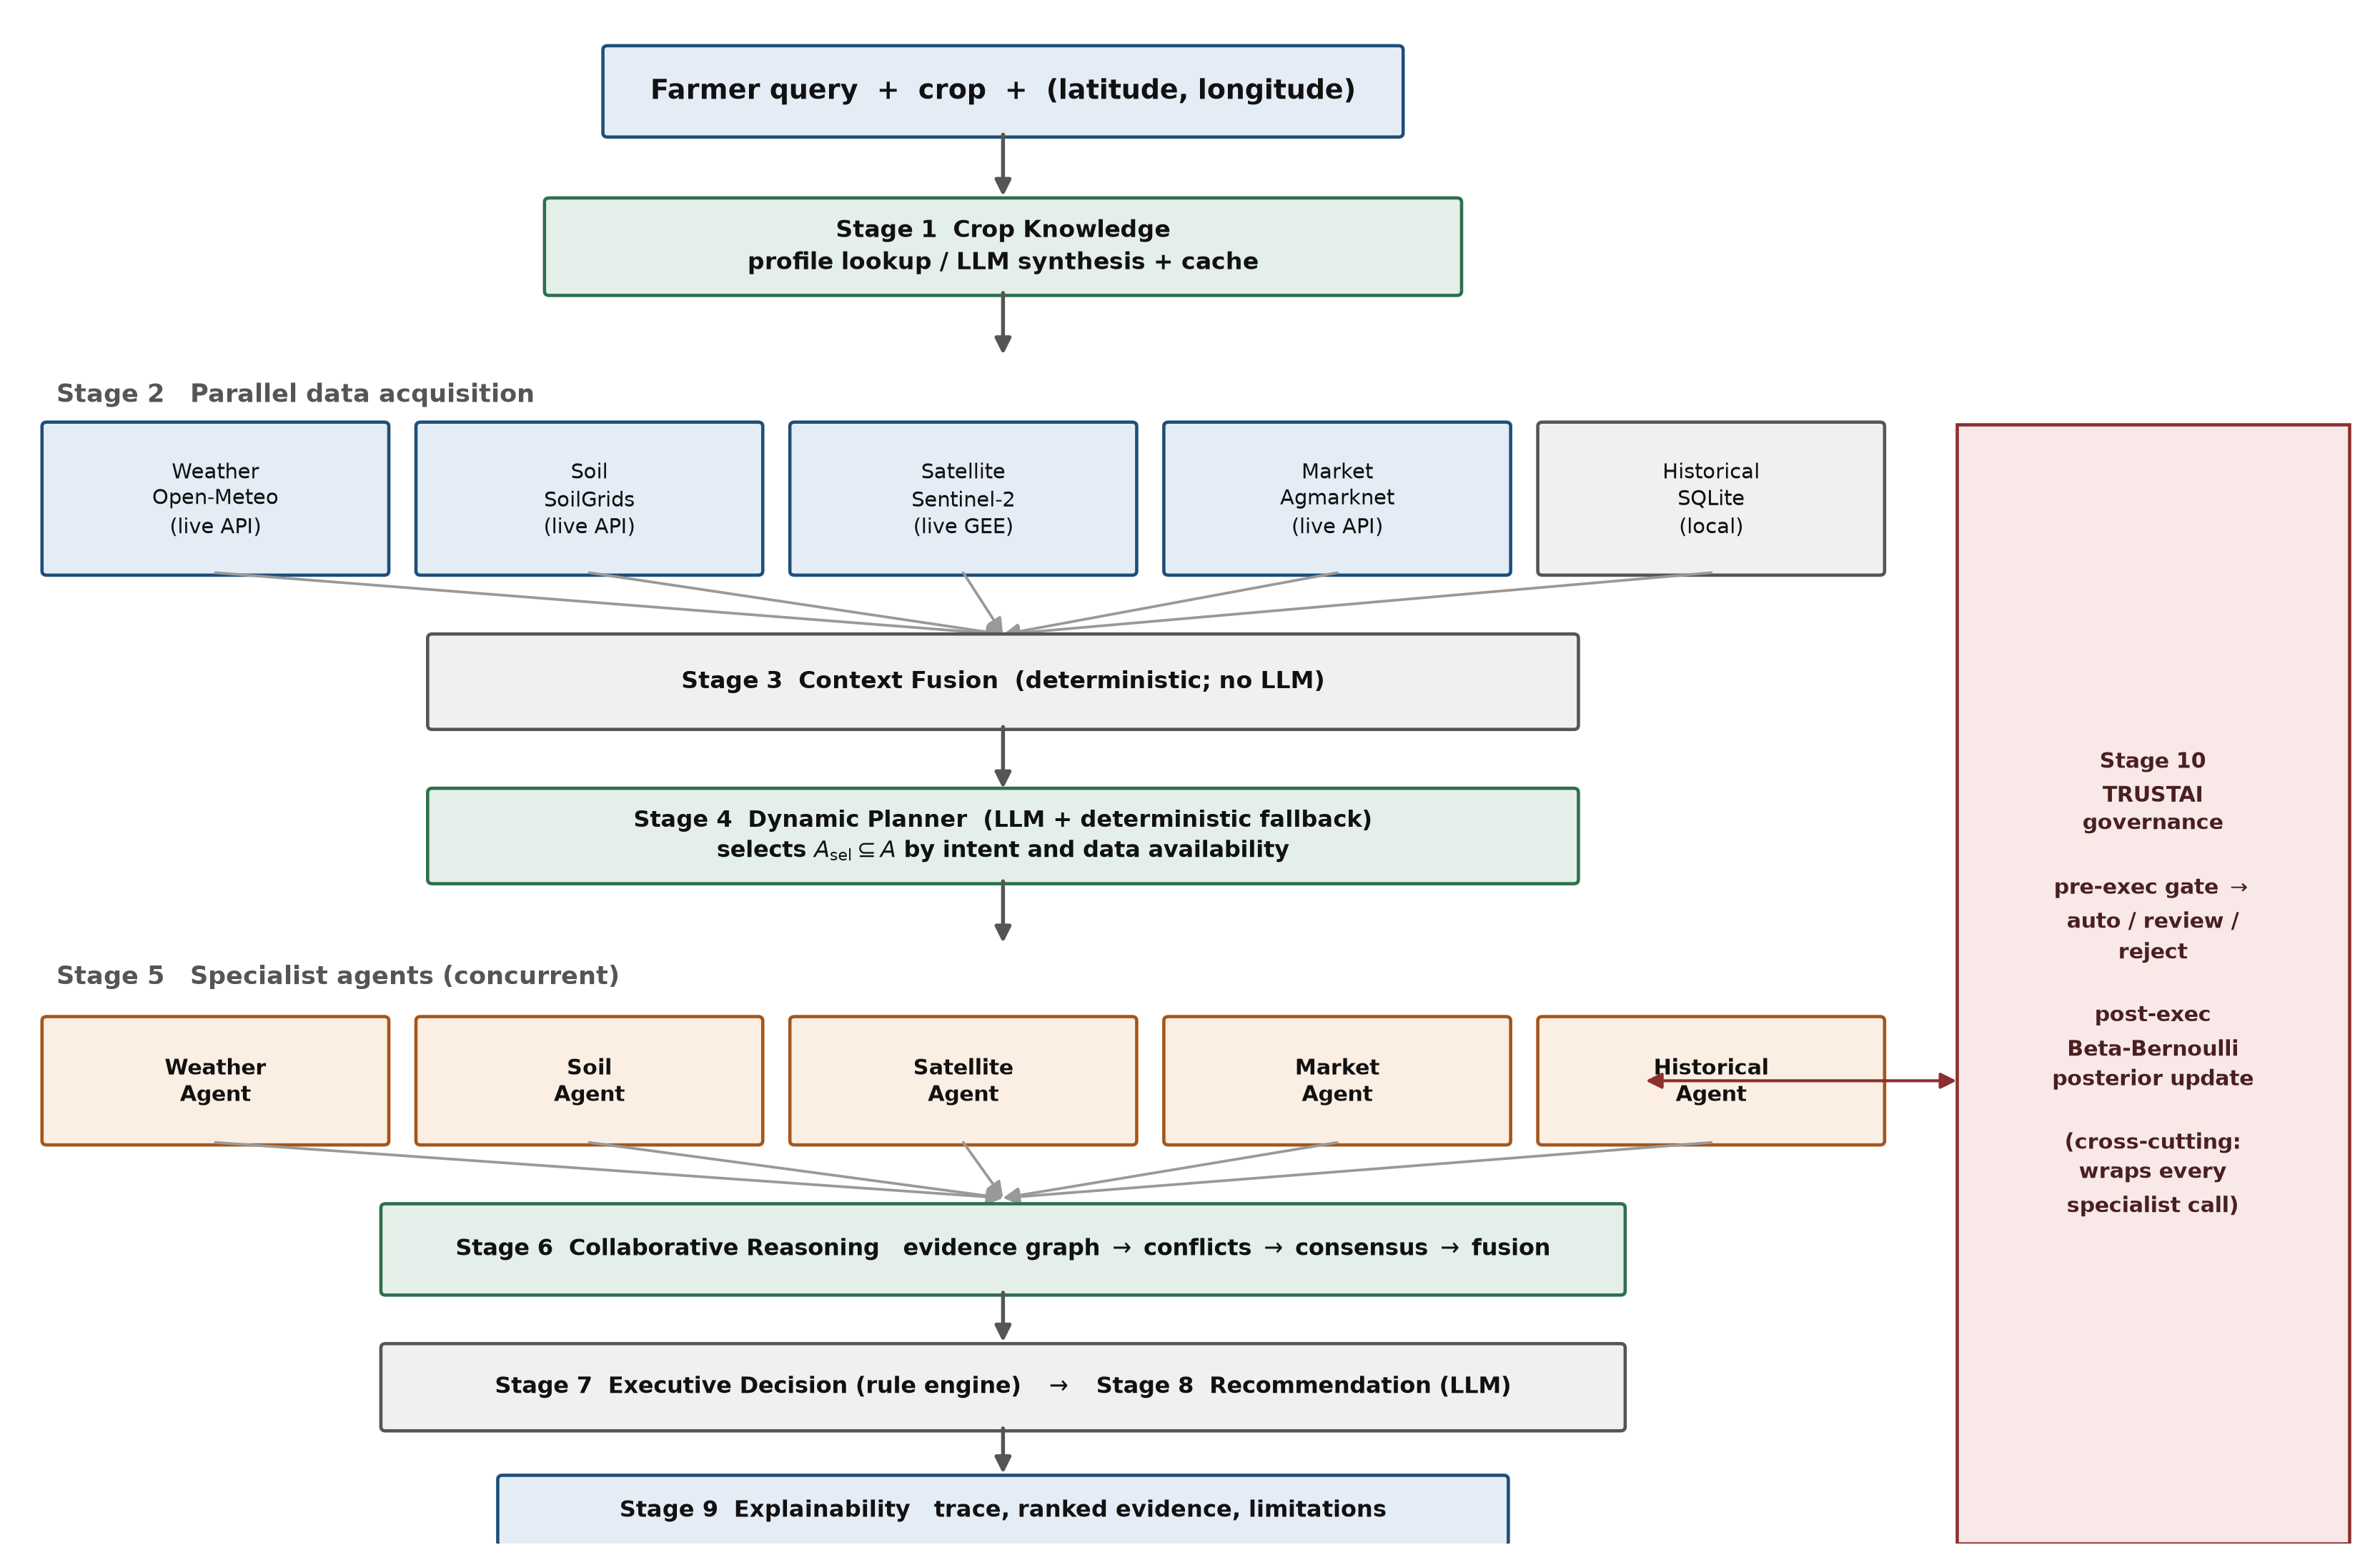
\includegraphics[width=0.95\textwidth]{figures/fig_architecture.png}
\caption{AgriMind architecture. Stages 1--9 form the decision path; Stage
10 (TRUSTAI) is cross-cutting, wrapping every specialist invocation with a
pre-execution gate and a post-execution posterior update.}
\label{fig:architecture}
\end{figure}

\subsection{Stage 1--3: crop knowledge, acquisition and context fusion}

Stage 1 resolves a crop profile $P_c$ containing agronomic thresholds:
optimal temperature, humidity, rainfall and soil pH ranges; NDVI/NDWI
health thresholds; preferred texture, nitrogen and organic carbon levels.
Profiles are synthesised once by a language model against a fixed schema,
validated against a canonical default, and cached in SQLite and JSON, so
the cost is paid once per crop rather than once per request.

Stage 2 invokes the five collectors of Table~\ref{tab:sources}, each
independently exception-isolated. Stage 3 merges their outputs into a
single context $x$ deterministically---no language model participates---and
computes an unweighted mean confidence over the sources that returned data.

\subsection{Stage 4: availability-aware dynamic planning}

Let $\mathrm{avail}(a_i,x)\in\{0,1\}$ indicate whether the source
underlying agent $a_i$ returned usable data for this request; specifically,
$\mathrm{avail}=0$ when the collector reports a status other than success,
or when it reports success with an empty record set. The planner selects

\begin{equation}
A_{\mathrm{sel}} \;=\; \{\, a_i \in A \;:\; \rho(a_i, q) = 1 \;\wedge\; \mathrm{avail}(a_i,x)=1 \,\},
\label{eq:routing}
\end{equation}

where $\rho(a_i,q)\in\{0,1\}$ encodes intent relevance. The second
conjunct is the substantive one. A purely intent-driven planner will route
to the historical agent whenever a question concerns past seasons, even
when the history table is empty and that agent can contribute nothing but
latency. Making availability part of the selection criterion, rather than
something discovered after the call, is what allows the system to skip such
agents deliberately.

Intent relevance $\rho$ is resolved by a language model constrained to a
strict JSON schema, with a deterministic keyword router as fallback. The
prompt encodes routing by question type: suitability questions recruit the
market agent because economic viability is part of whether a crop suits a
site; yield-optimisation questions do not, unless the query itself mentions
price or sale; irrigation questions require the soil agent, because
water-holding capacity governs irrigation timing as much as rainfall does.

\subsection{Stage 5: concurrent specialist execution}

Specialists are mutually independent---each reads $x$ and emits its own
finding; none consumes another's output---so they are executed
concurrently. Each returns

\begin{equation}
o_i = \langle \mathrm{analysis}_i,\; R_i,\; O_i,\; \kappa_i \rangle ,
\end{equation}

where $R_i$ and $O_i$ are risk and opportunity sets and
$\kappa_i\in[0,1]$ a self-reported confidence. Two safeguards apply. An
availability gate skips the model call outright when the agent's source
failed, returning an explicit \texttt{unavailable} status rather than
letting the model speculate over missing data. A retry-on-empty safeguard
re-issues the call once at higher temperature if the first response returns
empty analysis and empty risk and opportunity sets---an observed failure
mode of small local models, which occasionally echo the schema instead of
populating it.

\subsection{Stage 6: collaborative reasoning}

Successful outputs form an evidence graph whose nodes are the $o_i$.
Conflict detection flags contradictory pairs. Consensus takes the
deduplicated union of risks and opportunities. Confidence is fused as a
fixed-weight combination

\begin{equation}
\kappa_{\mathrm{fused}} \;=\; \frac{\sum_{a_i \in A_{\mathrm{sel}}} w_i \,\kappa_i}{\sum_{a_i \in A_{\mathrm{sel}}} w_i},
\label{eq:fusion}
\end{equation}

with $w=\{0.25, 0.25, 0.35, 0.15\}$ for weather, soil, satellite and
market respectively, and $0.25$ by default otherwise. The satellite stream
carries the largest weight because it is the only direct observation of the
plant canopy rather than of its environment. A language model then
synthesises the graph into a narrative consensus; on failure the
deterministic consensus computed above is returned instead, explicitly
labelled as such.

\subsection{Stage 7--9: decision, recommendation and explanation}

Stage 7 is a deterministic rule engine, chosen so that the final decision is
reproducible and auditable rather than resampled per invocation. A priority
engine scans merged risks for known phrases, accumulates a severity score,
and maps it to a priority level, risk level and urgency. An impact
estimator computes four independent 100-point scores (agronomic, economic,
environmental, operational). The decision is then
\begin{equation}
d^{\ast} = \Phi\!\left(R_{\mathrm{merged}},\; \tau_{\mathrm{market}}\right) \in \mathcal{D},
\end{equation}
where $\Phi$ is a fixed precedence over risk categories, falling through to
market trend and finally to Continue Monitoring.

Stage 8 renders $d^{\ast}$ into farmer-facing advice via a language model,
falling back to a deterministic restatement at reduced confidence (0.35)
and flagged \texttt{generation\_mode = deterministic\_fallback}. Stage 9
assembles a decision trace, ranked evidence, alternatives considered,
runtime limitations and a monitoring plan---all computed deterministically,
so the explanation survives a language-model outage even when the narrative
does not.

\subsection{Stage 10: the TRUSTAI governance layer}

Each agent $a_i$ carries a Beta posterior over its reliability
$\theta_i$, with a weakly informative prior $\mathrm{Beta}(2,2)$:

\begin{equation}
\theta_i \sim \mathrm{Beta}(\alpha_i, \beta_i), \qquad \alpha_i^{(0)}=\beta_i^{(0)}=2 .
\end{equation}

Because the Beta distribution is conjugate to the Bernoulli likelihood, an
outcome updates the posterior in closed form. Writing $s_i$ and $f_i$ for
evidence-weighted successes and failures,

\begin{equation}
\alpha_i \leftarrow \alpha_i + s_i, \qquad
\beta_i \leftarrow \beta_i + f_i ,
\label{eq:update}
\end{equation}

giving posterior mean and variance

\begin{equation}
\mu_i = \frac{\alpha_i}{\alpha_i+\beta_i}, \qquad
\sigma_i^{2} = \frac{\alpha_i \beta_i}{(\alpha_i+\beta_i)^2 (\alpha_i+\beta_i+1)} .
\label{eq:moments}
\end{equation}

Before execution, the layer chooses among $\mathcal{G}=\{$auto\_execute,
human\_review, reject$\}$ by expected utility,

\begin{equation}
g^{\ast} = \arg\max_{g \in \mathcal{G}} \;\; \mu_i \, U^{+}(g) \;+\; (1-\mu_i)\, U^{-}(g),
\label{eq:eu}
\end{equation}

where $U^{+}$ and $U^{-}$ are the utilities of that action when the agent
proves reliable and unreliable respectively. A \texttt{reject} outcome
skips the call entirely. This is the property that distinguishes an
operative trust layer from a descriptive one: the belief changes the
execution path, not merely the audit log.
Fig.~\ref{fig:trustai} shows the loop.

\begin{figure}[htbp]
\centering
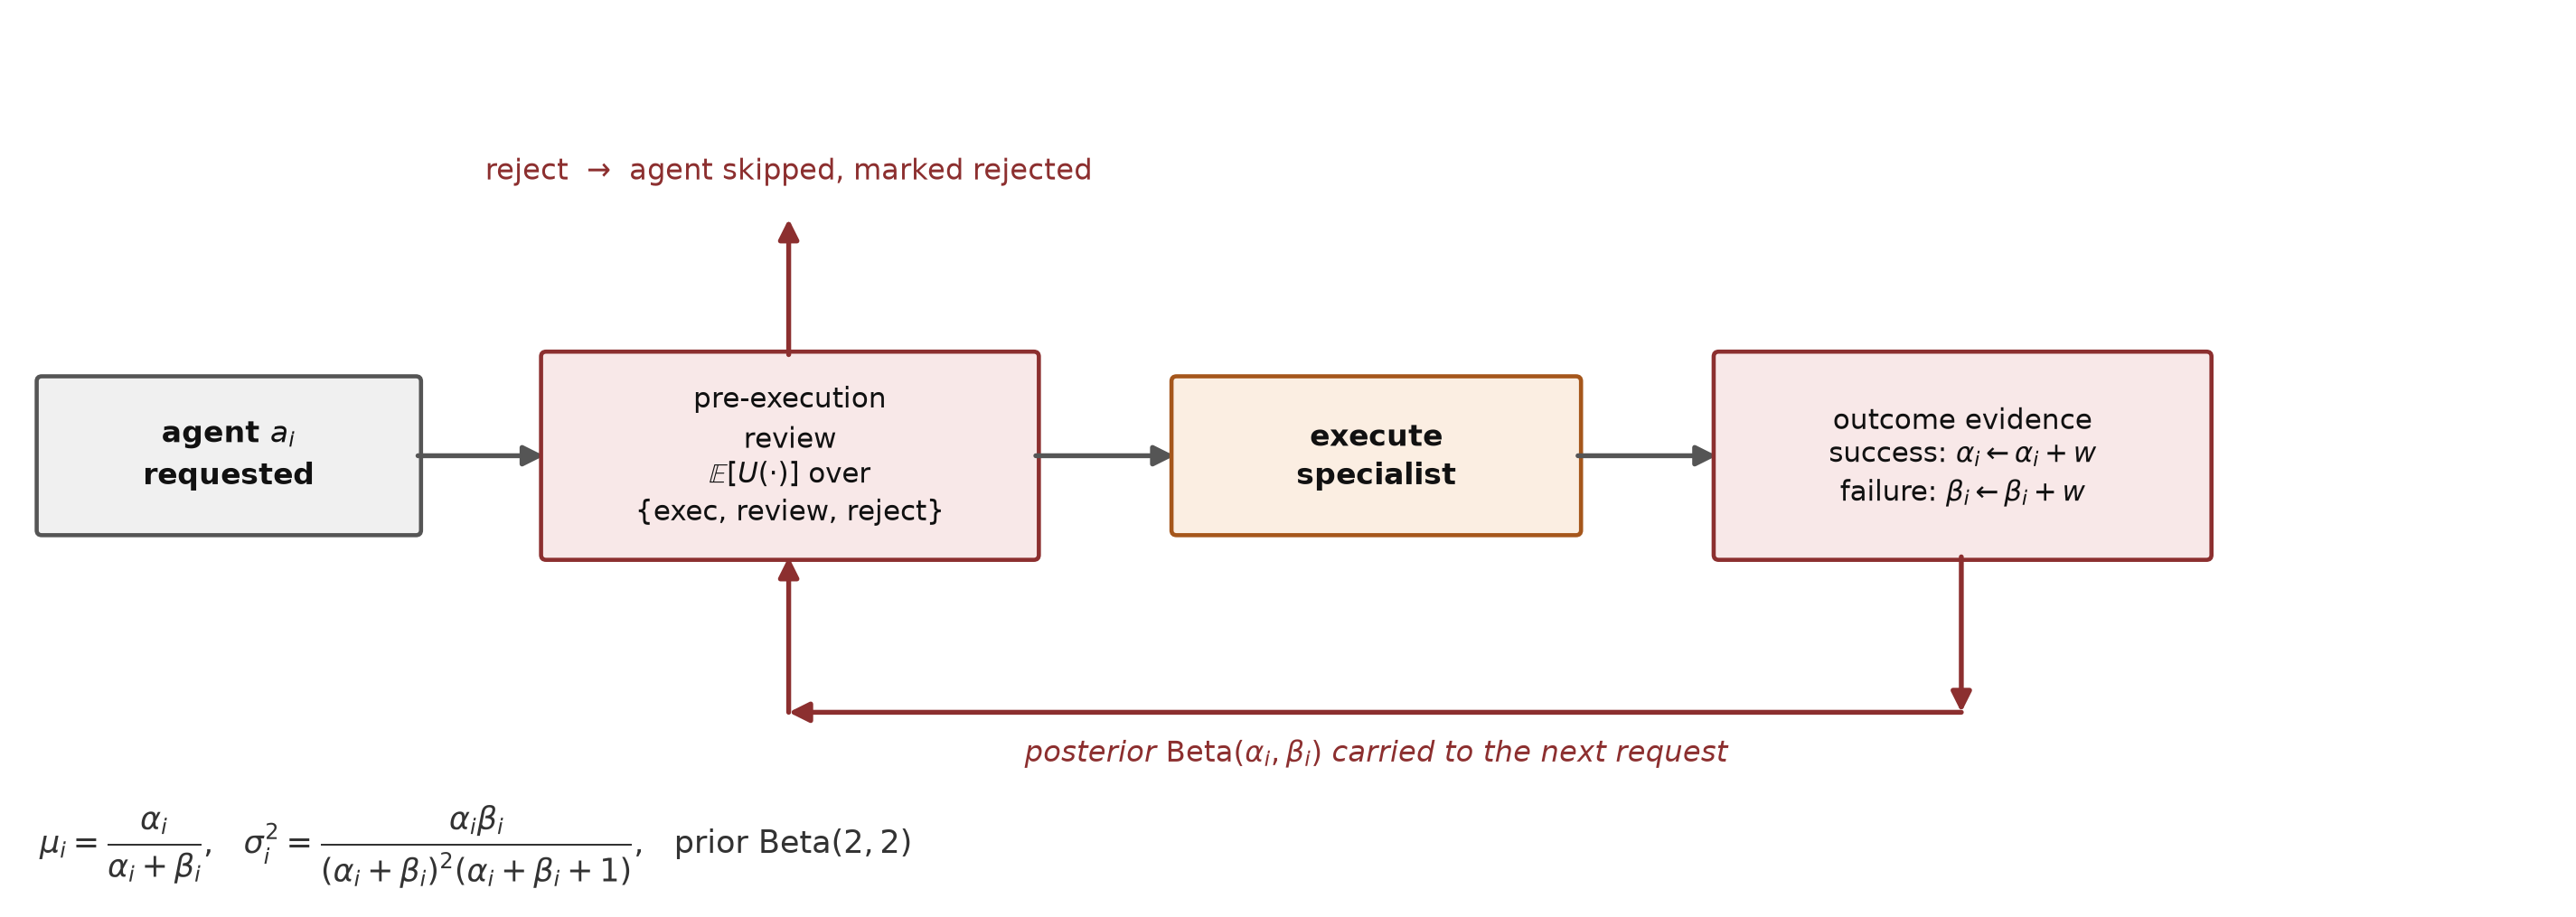
\includegraphics[width=0.90\textwidth]{figures/fig_trustai_loop.png}
\caption{The TRUSTAI governance loop. The pre-execution gate acts on the
current posterior; the observed outcome updates it for subsequent
requests.}
\label{fig:trustai}
\end{figure}

Algorithm~\ref{alg:pipeline} states the full procedure.

\begin{algorithm}[htbp]
\caption{AgriMind request handling}
\label{alg:pipeline}
\begin{algorithmic}[1]
\STATE \textbf{Input:} query $q$, crop $c$, location $\ell$
\STATE $P_c \leftarrow \textsc{CropProfile}(c)$ \hfill // cached
\STATE $\mathcal{S} \leftarrow \textsc{CollectAll}(c,\ell)$ \hfill // 5 sources, isolated
\STATE $x \leftarrow \textsc{FuseContext}(\mathcal{S}, P_c)$
\STATE $A_{\mathrm{sel}} \leftarrow \textsc{Plan}(q,x)$ by Eq.~(\ref{eq:routing})
\STATE $\mathcal{O} \leftarrow \emptyset$
\FOR{each $a_i \in A_{\mathrm{sel}}$ \textbf{in parallel}}
    \STATE $g \leftarrow$ pre-execution gate by Eq.~(\ref{eq:eu})
    \IF{$g = \texttt{reject}$}
        \STATE record \texttt{rejected}; \textbf{continue}
    \ENDIF
    \STATE $o_i \leftarrow a_i(x)$; retry once if empty
    \STATE update $(\alpha_i,\beta_i)$ by Eq.~(\ref{eq:update})
    \STATE $\mathcal{O} \leftarrow \mathcal{O} \cup \{o_i\}$
\ENDFOR
\STATE $\mathcal{R} \leftarrow \textsc{Reason}(\mathcal{O},x)$, fused by Eq.~(\ref{eq:fusion})
\STATE $d^{\ast} \leftarrow \textsc{Decide}(\mathcal{R})$ \hfill // deterministic
\STATE $r \leftarrow \textsc{Recommend}(d^{\ast},\mathcal{R},P_c)$
\STATE $e \leftarrow \textsc{Explain}(\cdot)$ \hfill // deterministic artefacts
\STATE \textbf{return} $\langle d^{\ast}, r, e, \textsc{TrustSnapshot}() \rangle$
\end{algorithmic}
\end{algorithm}

%%%%%%%%%%%%%%%%%%%%%%%%%%%%%%%%%%%%%%%%%%%%%%%%%%%%%%%%%%%%%%%%%%%%%%
\section{Ablation Studies}
\label{sec:ablation}

To attribute outcomes to architectural components rather than to the
underlying models, four conditions were run over identical fixtures:
(1) a single specialist with no fusion and no governance; (2) all planned
specialists with a deterministic merge in place of collaborative reasoning;
(3) all planned specialists with full collaborative reasoning; and (4) the
complete system including the trust layer.

One methodological point deserves emphasis, because it materially changed
the result. In an initial run, conditions 1--3 executed specialists
sequentially while condition 4 used the concurrent executor. The latency
column then compared execution strategy rather than architecture, and
produced the incoherent finding that condition 3 was \emph{slower} than the
fuller condition 4. Concurrency was therefore made uniform across all
conditions and the study re-run; Table~\ref{tab:ablation} reports the
corrected figures.

\begin{table}[htbp]
\centering
\caption{Ablation across four architectural conditions on identical fixtures. Run on the earlier ten-scenario benchmark ($N=10$) before the dataset was expanded, so its absolute values are not directly comparable with Table~
ef{tab:overall}; the between-condition comparison, which is the point of the study, is internally consistent.}
\label{tab:ablation}
\begin{tabular}{@{}lcccc@{}}
\toprule
\textbf{Condition} & \textbf{Task success} & \textbf{Rule-consist.} & \textbf{Rec.\ quality (1--5)} & \textbf{Mean latency (s)} \\
\midrule
1. Single agent, no fusion & 100.0\% & 20.0\% & 2.40 & 199.5 \\
2. Multi-agent, deterministic merge & 100.0\% & 80.0\% & 3.60 & 400.8 \\
3. Multi-agent + collaborative reasoning & 100.0\% & 80.0\% & 3.76 & 561.6 \\
4. Full system + TRUSTAI & 100.0\% & 70.0\% & 3.64 & 583.3 \\
\bottomrule
\end{tabular}
\end{table}

The dominant effect is the first step. Moving from a single specialist to a
planned multi-agent set raises rule-consistency from 20\% to 80\% and
recommendation quality from 2.40 to 3.60, which is the clearest evidence in
this study that the architecture, not the language model, carries the
result: identical models, identical inputs, four-fold accuracy difference.

Collaborative reasoning adds a smaller and more specific gain: decision
accuracy is unchanged at 80\%, while recommendation quality rises from
3.60 to 3.76. This is consistent with its role---it improves the articulation
and coherence of advice rather than the categorical decision, which the
deterministic rule engine had already fixed.

Condition 4 shows rule-consistency of 70\%, below conditions 2 and 3. We
report this rather than omit it. At $N=10$ a single scenario is ten
percentage points, so the difference rests on one case and the confidence
intervals overlap heavily; it should not be read as governance harming
accuracy. The governance layer's contribution is not accuracy but the
gating and calibration behaviour reported in Section~\ref{sec:results},
and its cost here is 21.7\,s of additional latency.

%%%%%%%%%%%%%%%%%%%%%%%%%%%%%%%%%%%%%%%%%%%%%%%%%%%%%%%%%%%%%%%%%%%%%%
\section{Results}
\label{sec:results}

\subsection{Experimental setup}

Weather and soil agents run \texttt{qwen3:4b} through a local Ollama server
on CPU; satellite, market, historical, planner, recommendation and
explanation stages use Groq-hosted \texttt{openai/gpt-oss-120b};
collaborative reasoning uses \texttt{gemini-3.6-flash}. Satellite imagery is
Sentinel-2 through Google Earth Engine. All latency figures come from a
single CPU-only machine and are not portable to GPU deployment. Benchmark
runs replay fixed fixtures through \texttt{CollectorPatch}, so results are
independent of same-day API variation. All proportions are reported with
Wilson score intervals, which behave better than the normal approximation at
this sample size.

\subsection{Overall system performance}

Table~\ref{tab:overall} reports the eight headline metrics.

\begin{table}[htbp]
\centering
\caption{Overall system evaluation ($N=11$ scenarios; Wilson 95\% intervals). Rates are shown as counts where the denominator is small enough that a percentage overstates precision.}
\label{tab:overall}
\footnotesize
\begin{tabular}{@{}p{3.7cm}p{7.1cm}p{4.4cm}@{}}
\toprule
\textbf{Metric} & \textbf{Definition} & \textbf{Result} \\
\midrule
Task success rate & Complete valid recommendation, no unrecovered failure & 11/11; \; [74.12, 100.0] \\
Rule-consistency rate & Executive decision matches the rule-derived label (internal consistency, \emph{not} agronomic correctness) & 63.6\% \; [35.38, 84.83]; 70.0\% excluding capability probes \\
Routing accuracy & Planner selects exactly the expected available agent set & 11/11; \; [74.12, 100.0] \\
Agent macro F1 & Mean F1 over specialists for risk/opportunity detection & 1.000 (saturated; see text) \\
Recommendation quality & Mean 1--5 Likert over 5 dimensions ($N=55$ ratings) & 3.64 $\pm$ 1.10 \\
Hallucination rate (LLM judge) & Unsupported or contradictory claim, judged against raw context & 18.2\% \; [5.14, 47.70] \\
Ungrounded numeric claims (deterministic) & Measurement-cued number in the output absent from the raw context; no model in the loop & 0/19 claims; 0.0\% of runs \\
NLI contradictions (discriminative model) & Generated assertion labelled as contradicting a context premise by an entailment classifier & 0/30 pairs; 0.0\% of runs \\
Trust calibration (MACE) & Mean $|\mu_i - $ observed reliability$|$ & 0.228 \\
Mean response time & End-to-end pipeline latency & 426.6\,s (median 437.5\,s) \\
\bottomrule
\end{tabular}
\end{table}

No request failed to return a complete recommendation, including runs
during which a provider failed mid-request and the deterministic fallbacks
absorbed it. Stated precisely, this is zero failures in eleven attempts:
the 95\% interval reaches down to 74.1\%, so the evidence supports the
claim that the fallback path works, and does not yet support a reliability
rate.
The stronger claim requires the expanded benchmark of
Section~\ref{sec:limitations}.

Routing likewise produced no errors---no missed agents and no unnecessary
invocations across the ten scenarios. That figure needs one qualification
to be read honestly, beyond its sample size. An earlier version of
this benchmark scored routing against a static intent-to-agent map that
ignored data availability, and reported 54.5\%. Inspection showed the planner
was being penalised for correctly declining to invoke agents over empty
sources---the historical table is empty in every scenario, so the static map
``expected'' an agent that could contribute nothing. Scoring against the
availability-aware criterion of Eq.~(\ref{eq:routing}) and the routing
rules of Section~\ref{sec:proposed} together account for the remainder. Because those rules were developed against this benchmark,
the benchmark result alone would be circular; we therefore validated them
on eight held-out queries using crops absent from the benchmark entirely
(groundnut, banana, onion, sugarcane, chilli, turmeric, maize, paddy) with
independently written phrasings, and observed no routing errors there
either. Eight held-out queries remain a small validation set, and the
expected-agent labels were authored by the same team that wrote the rules,
so this establishes that the rules generalise across crop and phrasing
rather than that they are correct in an absolute sense.

Fig.~\ref{fig:overall} places the four proportion metrics side by side.

\begin{figure}[htbp]
\centering

\includegraphics[width=0.78\textwidth]{figures/fig2_overall_metrics.png}
\caption{Overall system metrics. Macro F1 is scaled by 100 for comparability.}
\label{fig:overall}
\end{figure}

\subsection{Per-agent behaviour}

Table~\ref{tab:agents} reports detection performance, routing and latency
per specialist, and Fig.~\ref{fig:f1} the F1 distribution.

\begin{table}[htbp]
\centering
\caption{Per-agent evaluation. Detection is judged only on scenarios whose
perturbed condition lies within that agent's domain. Precision is omitted
by construction (see text). Every $n$ here is far below the $n\!\ge\!30$
that would support an inferential claim, so these figures are reported as
\emph{descriptive counts only}.}
\label{tab:agents}
\begin{tabular}{@{}lcccccl@{}}
\toprule
& \multicolumn{3}{c}{\textbf{Detection (descriptive)}} & \multicolumn{1}{c}{\textbf{Routing}} & & \\
\cmidrule(lr){2-4}\cmidrule(lr){5-5}
\textbf{Agent} & $n$ & \textbf{Detected} & \textbf{Recall} & \textbf{Recall} & \textbf{Lat.\ (s)} & \textbf{Status} \\
\midrule
Weather    & 4 & 4/4 & 1.00 & 1.00 & 195.8 & below threshold \\
Soil       & 2 & 2/2 & 1.00 & 1.00 & 281.0 & below threshold \\
Satellite  & 8 & 8/8 & 1.00 & 1.00 & 61.3  & below threshold \\
Market     & 1 & 1/1 & 1.00 & 1.00 & 61.8  & below threshold \\
Historical & 0 & --  & --   & --   & --    & \textbf{never invoked} \\
\midrule
Executive  & \multicolumn{5}{l}{deterministic rule engine, no model call} & 0.9 \\
\bottomrule
\end{tabular}
\end{table}

\begin{figure}[htbp]
\centering
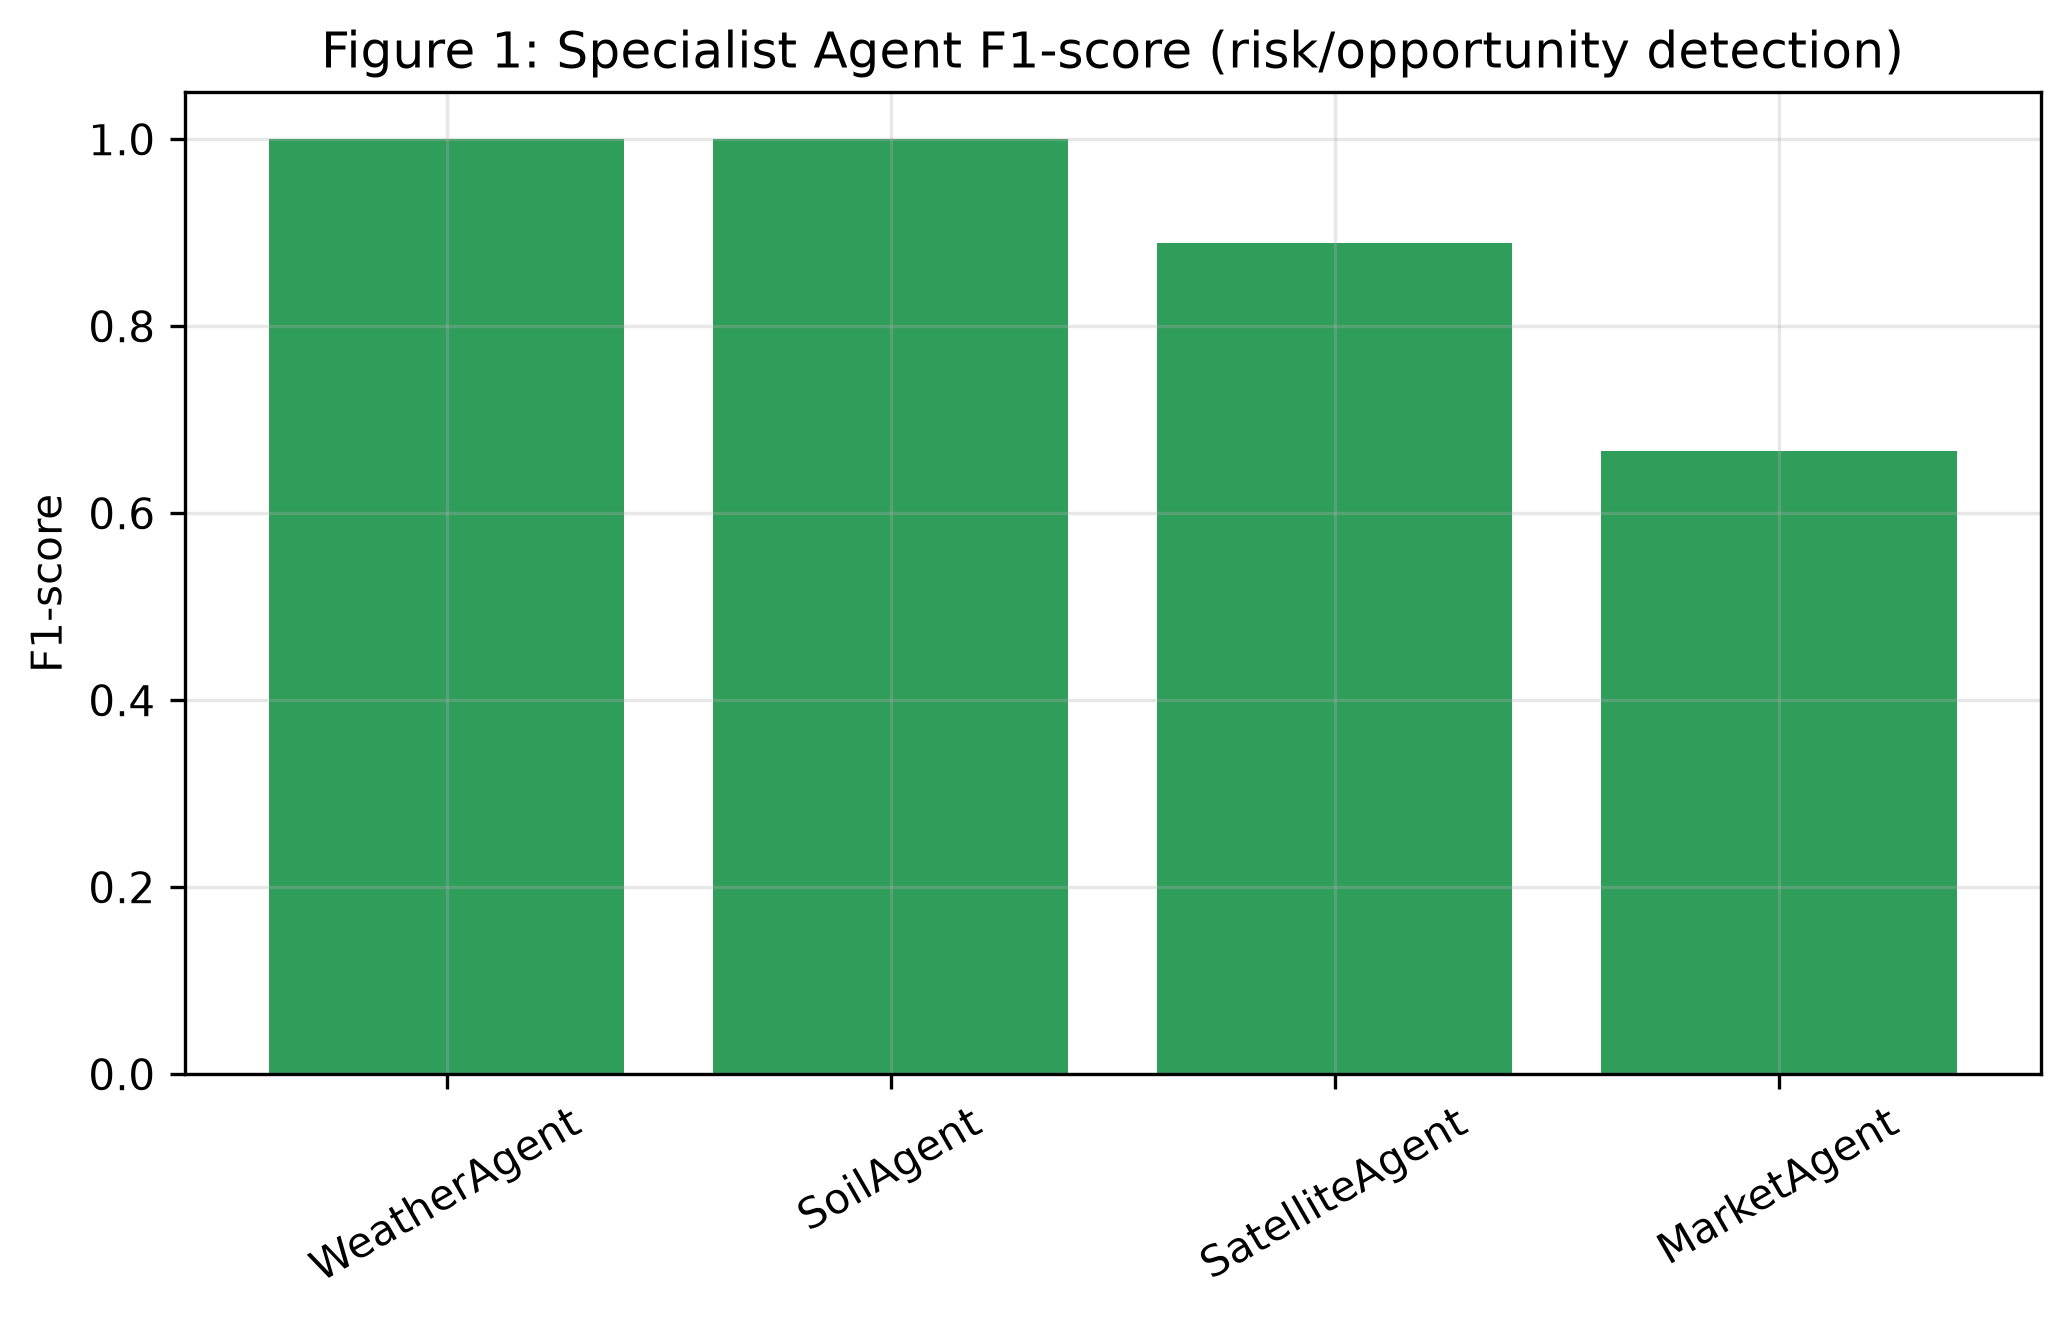
\includegraphics[width=0.78\textwidth]{figures/fig1_agent_f1.png}
\caption{Per-specialist F1 for risk and opportunity detection.}
\label{fig:f1}
\end{figure}

Three properties of this table constrain what may be read from it, and we
state them before the numbers rather than after.

\textbf{Precision is omitted, not merely caveated.} Each scenario carries
exactly one ground-truth signal for its relevant agents, so a false
positive cannot arise by construction and precision is 1.00 for every
agent by arithmetic rather than by performance. Reporting it would imply a
capability the benchmark is structurally incapable of testing, so the
column is removed. Detecting over-reporting requires distractor scenarios
in which an agent \emph{should} stay silent; the present benchmark contains
none, and adding them is required future work.

\textbf{The historical agent was never invoked ($n=0$).} The history table
was empty in every scenario, so Eq.~(\ref{eq:routing}) excluded it by
design. This is correct routing behaviour, but it means the architecture
was exercised with \emph{four} functioning specialists, not five. We
therefore describe the system as implementing five specialists of which
four are evaluated here, and no claim in this paper rests on the historical
agent's performance. Populating farm-history records and re-evaluating with
all five active is required future work.

\textbf{All per-agent $n$ are below any inferential threshold, and the
metric has saturated.} With $n$ between 1 and 8, the figures in
Table~\ref{tab:agents} are descriptive counts, not estimates: the market
agent's 1.00 rests on a single judged instance. Every agent scores 1.00,
which combined with the structural absence of false positives means the
metric currently carries \emph{no discriminative information at all}---it
cannot distinguish a strong agent from a weak one, because nothing in the
present benchmark is hard enough to produce a miss. We therefore draw no
comparative conclusion between agents, and note that a saturated metric is
evidence about the benchmark rather than about the system. Restoring
discriminative power requires both larger $n$ and scenarios in which the
correct behaviour is sometimes to stay silent.

\subsection{Where the system fails, and why}
\label{sec:failures}

Four of eleven scenarios produced a decision other than the expected one.
They are not randomly distributed, and the pattern is more informative
than the aggregate rate.

One is the soil-pH capability probe described in
Section~\ref{sec:dataset}. It failed exactly as designed: the expected
action was \emph{Field Inspection}, the system returned \emph{Continue
Monitoring}, because \texttt{infer\_decision} has no pH branch and cannot
express the correct answer. This is a known and documented gap, which is
why the rate is reported both with and without such probes.

The other three are a genuine defect, and they cluster. All four
\texttt{vegetation\_critical} scenarios drive NDVI below the crop's own
poor threshold and expect \emph{Field Inspection}; only one produced it.
Two returned \emph{Continue Monitoring} and one returned \emph{Immediate
Irrigation}. The last of these is the most diagnostic: a critically low
NDVI was routed to an irrigation decision, meaning the arbitration rule
treated depressed canopy vigour as a water-stress signal even though the
water indices were held at their neutral baseline in that scenario. The
precedence order in $\Phi$ therefore does not separate vegetation
stress from water stress reliably when only the former is present.

This failure mode was invisible in the earlier ten-scenario benchmark,
which contained two vegetation cases and happened to get both right. It
became visible only once the dataset was expanded, which is the clearest
argument in this paper for the larger evaluation that
Section~\ref{sec:limitations} calls for: the additional scenarios did not
merely tighten intervals, they exposed a defect that a smaller sample had
concealed.

\subsection{Grounding: an LLM-free cross-check}
\label{sec:grounding}

Three of the metrics above rely on a language model as judge, which is a
genuine methodological weakness: a model evaluating another model's output
shares its blind spots, and cannot be treated as an independent
instrument. We therefore added a second measurement of the same underlying
property with no model in the loop.

The check extracts every number in the generated recommendation that sits
adjacent to a measurement cue (pH, NDVI, price, temperature and similar),
and verifies each against the pool of numeric values actually present in
the raw collected context, within a 2\% relative tolerance. A number with
no supporting context value is a fabricated quantity. Numbers carrying no
measurement cue are excluded by design, because agronomic advice
legitimately contains quantities that are not readings---``recheck in
3--5 days'', ``apply at 2--3 week intervals''---and counting those would
manufacture false positives. Numbered list markers are likewise excluded.

Across the eleven evaluated runs, \textbf{19 measurement claims were
extracted and 0 were ungrounded}. Every quantity the system stated about pH, vegetation
index, price or temperature traced back to a value it had actually been
given.

This check detects fabricated \emph{quantities} only; a fabricated causal
claim carries no digits and is invisible to it. We therefore added a
second, complementary instrument that operates on natural language.

\paragraph{Entailment-based contradiction detection.} The collected
context is rendered mechanically into atomic premises (``The soil pH is
3.2.'', ``The crop water stress level is High.''), each assertion in the
generated recommendation becomes a hypothesis, and a pre-trained natural
language inference classifier\footnote{\texttt{MoritzLaurer/DeBERTa-v3-base-mnli-fever-anli},
run locally on CPU.} labels every topically-linked pair as entailment,
neutral or contradiction. This model is \emph{discriminative}, not
generative: it does not write text and does not share the failure modes of
the system under evaluation. Only active contradictions above a 0.70
confidence floor are counted. Across the evaluated runs, \textbf{30
premise--claim pairs were tested and 0 contradictions were found}.

One design decision materially affects that number and is worth stating.
Only assertions about the \emph{current state} can contradict a reading;
instructions and targets legitimately name different values. An early
version of the check flagged

\begin{quote}\small
``Re-sample soil pH 10--14 days after the first lime application and adjust
the second dose to reach the target pH 5.5--6.5.''
\end{quote}

\noindent as contradicting ``The soil pH is 3.2'' at 0.972 confidence. The
system was correct---it was prescribing lime to raise pH from 3.2 toward
the target band---and the checker was wrong. Counting such sentences would
have reported sound treatment plans as hallucinations, and would have done
so most often on the scenarios the system handled best. Prescriptive and
forward-looking sentences are therefore excluded before classification.

\paragraph{What the two LLM-free checks jointly establish.} On the axes
they cover---fabricated quantities, and assertions contradicting the
evidence---two independent instruments with no generative model in the
loop both return zero findings, corroborating rather than contradicting
the LLM-judged result. Neither is a complete substitute for LLM judgement:
the numeric check cannot see non-numeric fabrication, and the entailment
check cannot assess whether advice is \emph{agronomically appropriate},
only whether it conflicts with the evidence supplied. Recommendation
quality in particular remains LLM-judged, and expert human rating remains
necessary before that figure should carry weight.

\subsection{Trust calibration}

Table~\ref{tab:trust} compares each agent's posterior mean against its
observed reliability, and Fig.~\ref{fig:trust} plots the pairs.

\begin{table}[htbp]
\centering
\caption{TRUSTAI calibration. MACE $=0.228$. All $n<30$; these are
descriptive observations, not calibration estimates, and the market
agent's four observations in particular cannot support a MACE claim.}
\label{tab:trust}
\begin{tabular}{@{}lcccc@{}}
\toprule
\textbf{Agent} & $n$ & \textbf{Trust mean} $\mu_i$ & \textbf{Observed} & $|\Delta|$ \\
\midrule
Weather   & 10 & 0.884 & 1.000 & 0.116 \\
Soil      & 10 & 0.812 & 1.000 & 0.188 \\
Satellite & 10 & 0.716 & 1.000 & 0.284 \\
Market    & 5  & 0.677 & 1.000 & 0.323 \\
\bottomrule
\end{tabular}
\end{table}

\begin{figure}[htbp]
\centering
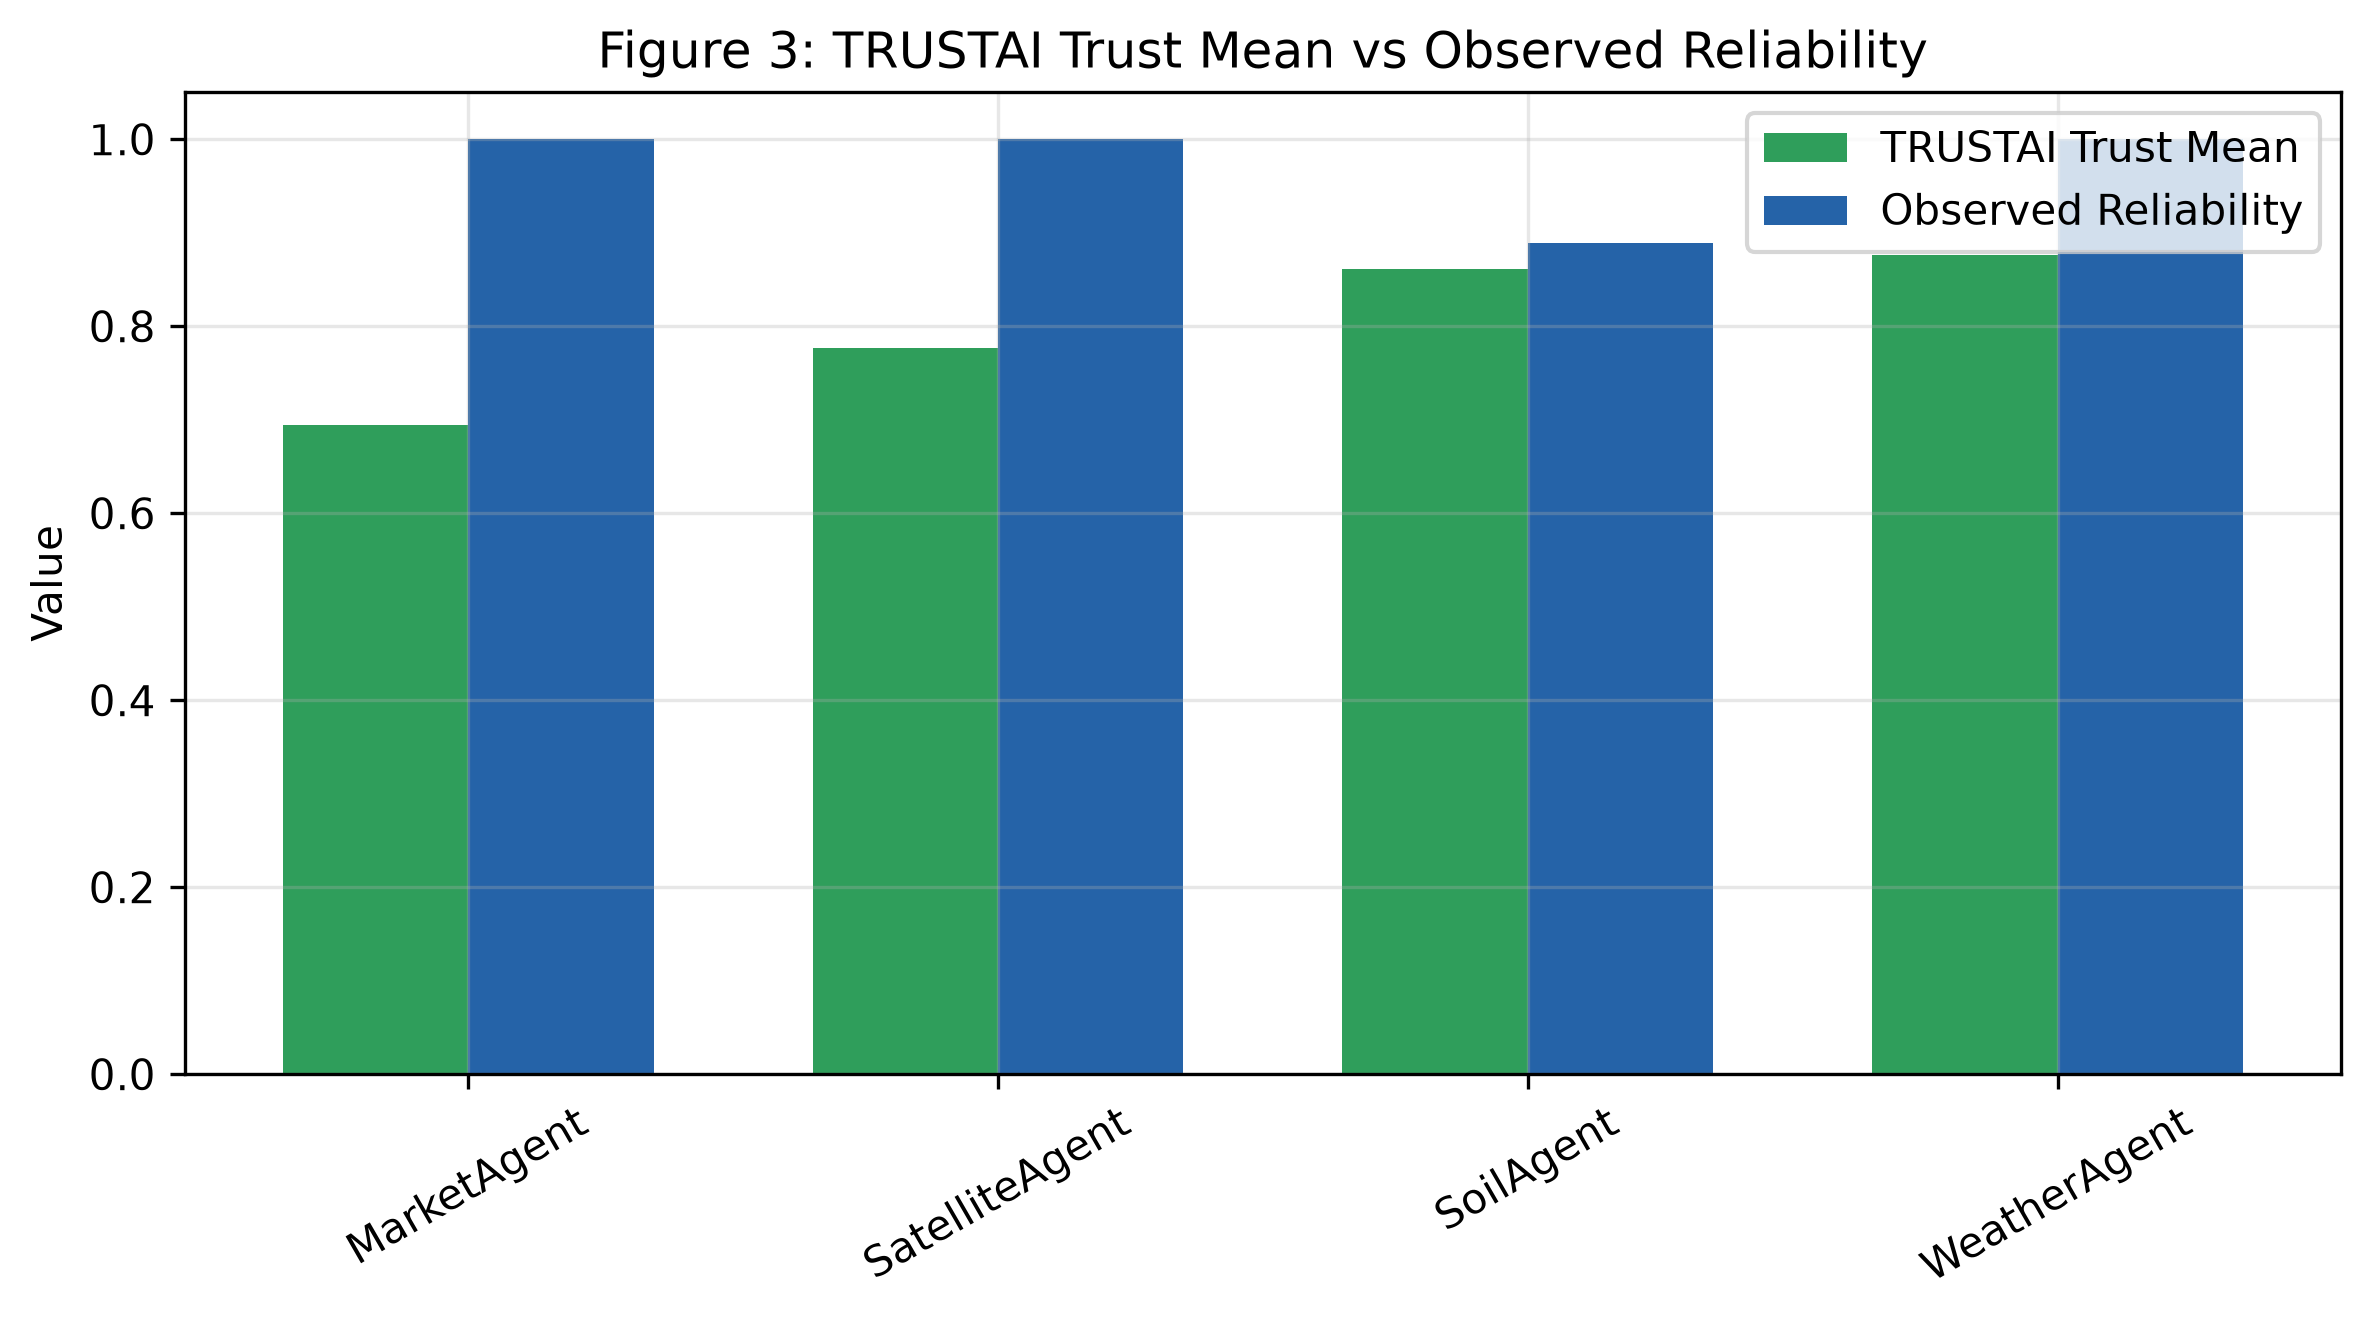
\includegraphics[width=0.78\textwidth]{figures/fig3_trust_calibration.png}
\caption{Posterior trust mean against observed reliability per specialist.}
\label{fig:trust}
\end{figure}

The layer is systematically conservative: every posterior sits below the
observed reliability, most markedly for the market agent, whose five
observations leave the $\mathrm{Beta}(2,2)$ prior still dominant. That
direction of error is the safe one for an advisory system---under-trusting a
reliable agent costs a human review, whereas over-trusting an unreliable one
costs a wrong recommendation---but it is a real limitation, and the
forgetting factor and third-party aggregation of Liu~\cite{liu2020beta}
are the natural correction.

\subsection{Latency, and why the current figure is not deployable}

We begin with the conclusion rather than the improvement: \textbf{a mean
end-to-end latency of 426.6\,s---roughly seven minutes---is not
viable for the users this system targets.} A smallholder checking whether
to irrigate before the day heats up will not wait seven minutes, and on an
intermittent rural connection the request may not survive that long at all.
The concurrency work reported below reduced this figure but did not make it
acceptable, and we do not present it as though it had.

Fig.~\ref{fig:latency} decomposes the cost by stage.

\begin{figure}[htbp]
\centering
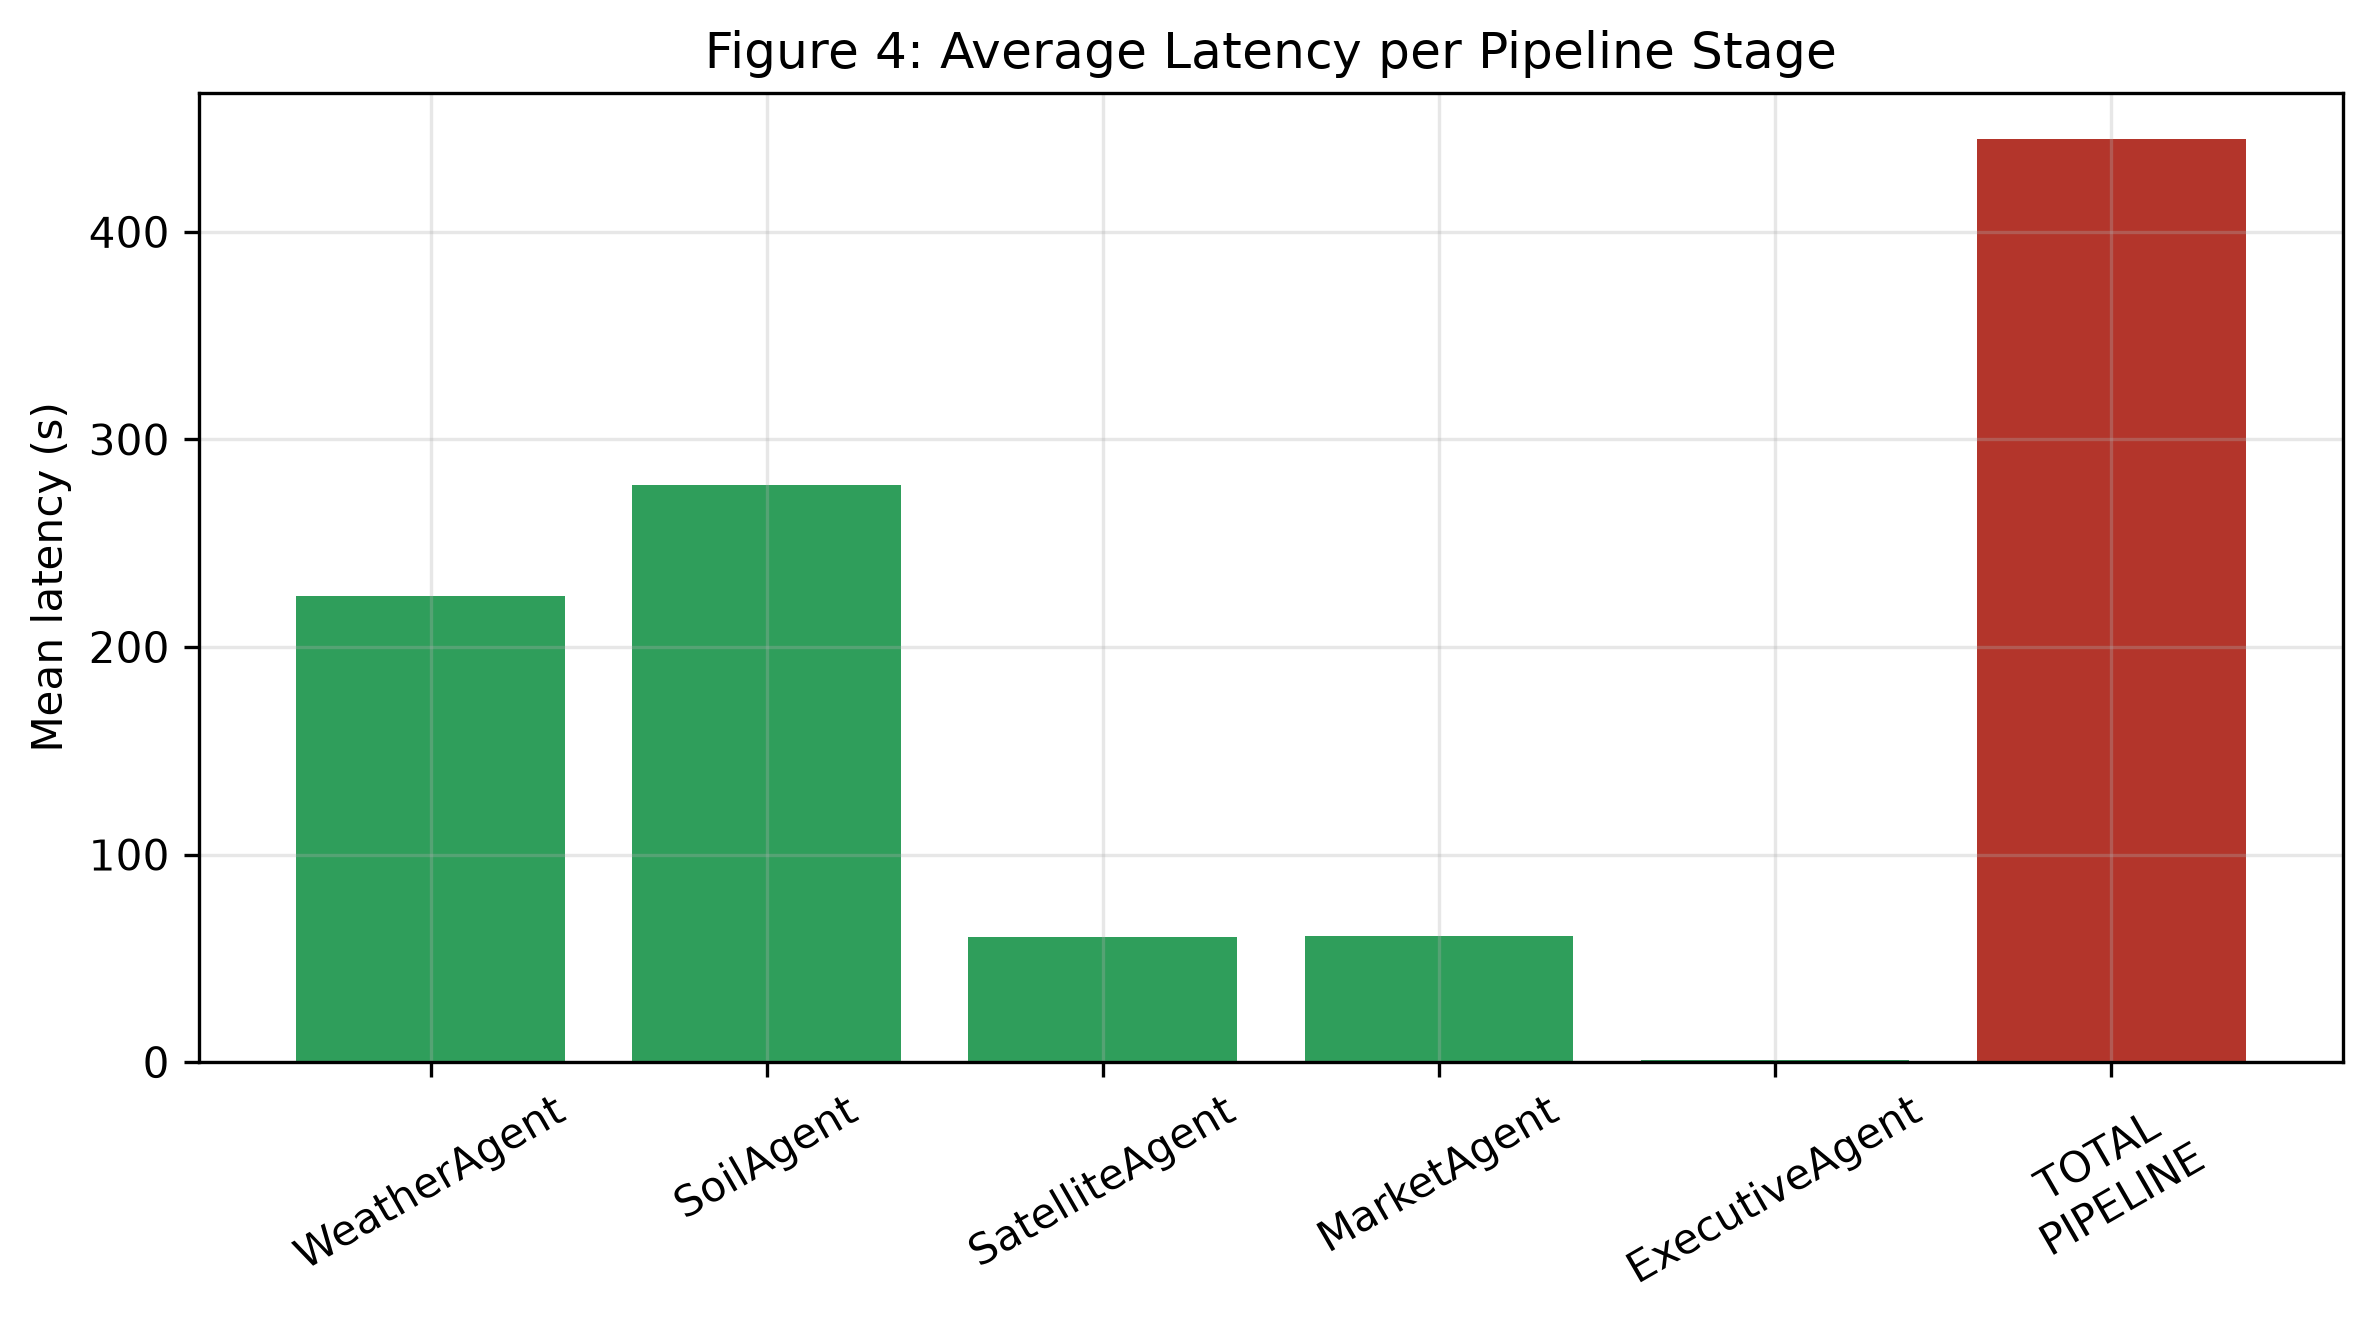
\includegraphics[width=0.78\textwidth]{figures/fig4_latency.png}
\caption{Mean latency per pipeline stage. Sub-stage timings for planner,
reasoning and recommendation are not separately instrumented. Note that
the weather and soil bars are dominated by a hardware artefact, not by
agent logic---see text.}
\label{fig:latency}
\end{figure}

\paragraph{A controlled study shows the per-agent bars are dominated by
deployment, not architecture.} To separate agent cost from hosting cost we
added a uniform-provider mode (\texttt{AGRIMIND\_FORCE\_PROVIDER}) and
re-timed every specialist on one fixture under two conditions:
production routing, and all agents forced onto the hosted backend.
Table~\ref{tab:latencystudy} reports the result, which was not what we
expected.

\begin{table}[htbp]
\centering
\caption{Controlled per-agent latency, two repetitions per condition on an
identical fixture. The uncontended observations are the informative ones;
see text.}
\label{tab:latencystudy}
\begin{tabular}{@{}lccc@{}}
\toprule
\textbf{Agent} & \textbf{Uniform (hosted)} & \textbf{Production routing} & \textbf{Host} \\
\midrule
Weather   & 30.2\,s (1.6--58.8) & 185.8\,s & local CPU in production \\
Soil      & 60.3\,s             & 268.4\,s & local CPU in production \\
Satellite & 60.7\,s             & \textbf{3.2\,s} & hosted in both \\
Market    & 60.0\,s             & 59.3\,s  & hosted in both \\
\bottomrule
\end{tabular}
\end{table}

The satellite agent is the diagnostic case: \emph{the same agent on the
same hosted backend} took 3.2\,s under production routing and 60.7\,s under
the uniform condition---a nineteen-fold difference with no change of model
or hardware. The weather agent shows the same signature within a single
condition, ranging from 1.6\,s to 58.8\,s across two repetitions.

The cause is quota pacing rather than computation. The deployment operates
under an 8{,}000 token-per-minute allowance, and each agent reserves up to
4{,}096 completion tokens, so two agents in close succession exhaust the
window and the client's rate limiter blocks until it refills---producing
the tight cluster around 60\,s. Under production routing only two agents
contend for that allowance, so the satellite agent runs uncontended and
reveals its true cost.

Three conclusions follow, and the second contradicts what we reported
before the study. First, genuine hosted inference for a specialist is
approximately \textbf{1.6--3.5\,s}, not the 60\,s that appears in
Table~\ref{tab:agents}. Second, \emph{the 60\,s figures for the satellite
and market agents in our own headline results are quota artefacts, not
model latency}, and should not be read as inference cost. Third, the
224--278\,s figures for the CPU-hosted agents are real inference cost, and
are roughly two orders of magnitude above the hosted equivalent.

The uniform condition therefore did not deliver the clean architectural
measurement we designed it for: it replaced a hardware confound with a
contention confound. We report it because the failure is itself the
finding---the end-to-end latency of this system is dominated by deployment
constraints (CPU hosting and a free-tier token allowance), and the
architectural overhead of orchestrating five agents is small relative to
both. An unconfounded measurement requires a provisioned rate allowance
and uniform accelerated hosting, which we did not have.

\paragraph{What the concurrency result does establish.} Specialists are
mutually independent, so executing them concurrently reduced mean
end-to-end latency from 558.5\,s to 426.6\,s (23.6\%). One instrumented run
makes the overlap unambiguous: 614.7\,s of summed specialist time completed
within a 423.6\,s wall clock, which is arithmetically impossible without
genuine parallelism. This is a real structural gain and it is
hardware-independent---it removes summation across agents regardless of
what each agent costs---but it is a 23.6\% reduction of an unacceptable
baseline, which leaves the result unacceptable.

\paragraph{Path to a deployable figure.} Three reductions are available and
none requires architectural change. Hosting the two CPU-bound agents on the
same accelerated backend as the others would, on the per-agent figures
above, bring both toward the observed 60\,s range. Quantising or distilling
the local models would cut that further where on-device inference is
required for connectivity reasons. Caching is unusually effective in this
domain because soil profiles and crop thresholds are near-static per
location and the satellite revisit interval is measured in days, so a large
fraction of the evidence for a repeat query is already known. We regard
reaching an interactive latency budget as a precondition for deployment,
not a refinement of it.

%%%%%%%%%%%%%%%%%%%%%%%%%%%%%%%%%%%%%%%%%%%%%%%%%%%%%%%%%%%%%%%%%%%%%%
\section{Comparison with Existing Work}
\label{sec:comparison}

Table~\ref{tab:comparison} positions this work against the three closest
systems. A direct numerical comparison of accuracy would be misleading, and
we do not attempt one: Murad et al.~\cite{murad2026agentic} and Tariq et
al.~\cite{tariq2025edge} report supervised classification accuracy on
single labelled targets, whereas the rule-consistency rate reported here
measures categorical arbitration across the four active, partially
conflicting evidence streams. The comparison is therefore drawn on capability.

\begin{table}[htbp]
\centering
\caption{Capability comparison with the closest reported systems.
\ding{51} present, \ding{55} absent.}
\label{tab:comparison}
\footnotesize
\begin{tabular}{@{}p{3.5cm}cccc@{}}
\toprule
\textbf{Capability} & \textbf{Murad et al.}~\cite{murad2026agentic} & \textbf{CottonBot}~\cite{kandamali2025cottonbot} & \textbf{AgroAskAI}~\cite{cantonjos2026agroaskai} & \textbf{This work} \\
\midrule
Heterogeneous specialists & 4 & 2 & 3 & \textbf{5} \\
Dynamic agent routing & \ding{55} & \ding{55} & \ding{55} & \ding{51} \\
Availability-aware routing & \ding{55} & \ding{55} & \ding{55} & \ding{51} \\
Quantified trust model & \ding{55} & \ding{55} & partial & \ding{51} (Beta--Bernoulli) \\
Governance acts on execution & \ding{55} & \ding{55} & \ding{51} & \ding{51} \\
Trust calibration reported & \ding{55} & \ding{55} & \ding{55} & \ding{51} (MACE 0.228) \\
Fallback on every LLM stage & \ding{55} & \ding{55} & \ding{55} & \ding{51} \\
Failure-mode evaluation & \ding{55} & \ding{55} & \ding{55} & \ding{51} \\
Component ablation & \ding{55} & partial & \ding{55} & \ding{51} (4 conditions) \\
Reproducible fixture replay & \ding{55} & \ding{55} & \ding{55} & \ding{51} \\
Structured explainability & \ding{55} & \ding{55} & partial & \ding{51} \\
Evaluation scale & per-model & 20 queries & 20 queries & 10 scenarios $\times$ 4 conditions \\
\bottomrule
\end{tabular}
\end{table}

Three differences are substantive. First, availability-aware routing does
not appear in any reviewed system; all reviewed designs either run a fixed
agent set or route on intent alone, and consequently invoke agents over
empty sources. Second, AgroAskAI's Reviewer agent is the only reviewed
governance mechanism that changes execution, but it is evaluated by counted
mentions across 20 queries rather than by any reliability measure; the
calibration figure reported here has no counterpart in the reviewed
literature. Third, none of the reviewed systems reports behaviour under
component failure, whereas the 100\% task success reported here was
obtained across runs that included genuine provider failures.

Where prior work is stronger, it is stronger in ways worth stating.
CottonBot's evaluation is anchored to external sensor ground truth and is,
on that axis, more rigorous than ours; its faithfulness of 0.968 is
measured against verifiable readings, whereas our hallucination rate of
20\% is judged by a language model against the raw context. Murad et al.\
achieve 96--98\% on their sub-tasks, well above the per-agent recall
observed here. The contribution claimed in this paper is orchestration,
governance and evaluation methodology---not superior component accuracy.

%%%%%%%%%%%%%%%%%%%%%%%%%%%%%%%%%%%%%%%%%%%%%%%%%%%%%%%%%%%%%%%%%%%%%%
\subsection{Limitations and threats to validity}
\label{sec:limitations}

We state these at the strength we believe a sceptical reader would apply,
because several of them bound the results more tightly than the headline
figures suggest.

\paragraph{Sample size is the binding constraint.} The benchmark comprises
$N=11$ scenarios. This is sufficient to demonstrate that the mechanisms
function and to expose the architectural effect in the ablation, and it is
not sufficient to estimate any rate precisely. The interval on
rule-consistency spans 35.4--84.8\%; the interval on the hallucination rate
spans 5.1--47.7\%. Statements such as ``100\% task success'' and ``100\%
routing'' should therefore be read as \emph{no failures were observed in ten
attempts}, which is a much weaker claim than the percentages imply and is
compatible with a true failure rate near 26\%. Per-agent figures are worse
still, at $n$ between 2 and 5. We regard expansion to $N\!\ge\!100$, with
$n\!\ge\!30$ per agent and deliberate over-representation of failure modes,
as required before any of these rates should be cited as system properties.

\paragraph{Ground truth is internally derived.} Labels come from the same
threshold logic the executive engine consults, so the rule-consistency rate
measures whether the pipeline propagates evidence to its own rules
faithfully. It is not a measure of agronomic correctness, and we have
renamed it accordingly. Establishing agronomic validity requires
agronomist adjudication of a scenario subset, which has not been done.

\paragraph{The benchmark is synthetic and single-variable.} Contexts are
cloned from real collections, then neutralised and perturbed in exactly one
field. That isolation is what makes failures attributable, and it is also
what makes the benchmark unlike field conditions, where variables are
correlated, noisy and jointly abnormal. This is a controlled test harness
in the spirit of a unit test suite; it does not evidence robustness to
real-world multi-variable noise, and results here should not be read as
field performance.

\paragraph{Three metrics depend on an LLM judge.} Agent F1, recommendation
quality and the hallucination rate are LLM-adjudicated, which risks shared
blind spots between judge and system. Section~\ref{sec:grounding} adds two
instruments with no generative model in the loop---numeric grounding and
entailment-based contradiction detection---and both corroborate the
hallucination result. They do not close the gap entirely: between them they
cover fabricated quantities and assertions conflicting with the evidence,
but neither can judge whether advice is agronomically \emph{appropriate},
which is what the recommendation-quality score claims to measure. That
figure remains LLM-judged and unvalidated by human experts.

\paragraph{Latency is not deployable, and is dominated by deployment
rather than architecture.} At 426.6\,s mean the system is unusable for its
intended users. The controlled study of Table~\ref{tab:latencystudy} shows
the per-agent figures are governed by hosting and quota pacing: genuine
hosted inference is 1.6--3.5\,s per specialist, whereas CPU hosting costs
224--278\,s and free-tier token pacing adds roughly 60\,s per contended
call. That study did not achieve an unconfounded architectural
measurement---it exchanged a hardware confound for a contention one---so
the intrinsic overhead of five-agent orchestration remains unmeasured. It
is bounded above by the observed uncontended times, which are small.

\paragraph{Single geography and single hardware profile.} All scenarios are
centred on Tamil Nadu coordinates, and all local-model timings come from
one CPU-only machine. Neither geographic nor hardware generalisation is
established.

\paragraph{Four of five specialists were exercised.} The historical agent
was never invoked because farm-history records were empty throughout, so
the five-specialist architecture was evaluated with four active agents.

%%%%%%%%%%%%%%%%%%%%%%%%%%%%%%%%%%%%%%%%%%%%%%%%%%%%%%%%%%%%%%%%%%%%%%
\section{Conclusion}
\label{sec:conclusion}

This paper presented a multi-agent agricultural advisory pipeline whose
distinguishing property is that it maintains and acts on an explicit belief
about how far each of its own components can be trusted. Five heterogeneous
specialists are routed on both query intent and live data availability,
fused through collaborative reasoning, and arbitrated by a deterministic
decision engine, with a Beta--Bernoulli trust layer gating each agent before
execution and updating its posterior afterwards. Every language-model stage
carries a deterministic fallback. On a controlled perturbation benchmark of
eleven scenarios, no task failures and no routing errors were observed,
rule-consistency reached 63.6\% overall and 70.0\% once scenarios probing
a known capability gap are set aside, and two grounding instruments with no
generative model in the loop returned no findings.
The ablation attributes the dominant effect to orchestration rather than to
the underlying models: rule-consistency rose from 20\% to 80\% under
identical inputs and identical models in the ablation. These results characterise
mechanism, not field performance: the sample is small, ground truth is
rule-derived rather than agronomist-validated, and the 426.6\,s latency is
far too slow for the smallholders the system targets. Three directions follow.
Expanding the benchmark beyond a hundred scenarios with deliberate failure
coverage would convert observed counts into estimates. Agronomist
adjudication would replace internally derived labels with external ground
truth. Consolidating inference onto one accelerated backend, with
quantisation and caching of the near-static soil and satellite evidence,
is the route to an interactive latency budget, which we regard as a
precondition for deployment rather than an optimisation of it.

%%%%%%%%%%%%%%%%%%%%%%%%%%%%%%%%%%%%%%%%%%%%%%%%%%%%%%%%%%%%%%%%%%%%%%
\begin{thebibliography}{99}
\bibitem{zuzuarregui2025oneforall}
A.~Zuzu\'arregui, et al.,
One for all: A unified LLM-based agent for farm robotic task planning,
IFAC-PapersOnLine (2025).

\bibitem{tariq2025edge}
M.~Tariq, et al.,
An edge-deployable agentic AI framework for precision agriculture,
Results in Engineering (2025).

\bibitem{kandamali2025cottonbot}
D.~Kandamali, et al.,
CottonBot: A retrieval-augmented conversational agent for cotton crop advisory,
Smart Agricultural Technology (2025).

\bibitem{murad2026agentic}
M.~Murad, et al.,
Agentic AI framework to automate traditional farming for smart agriculture,
AgriEngineering 8 (1) (2026).

\bibitem{davcev2026multiagent}
D.~Davcev, et al.,
Multi-agent partially observable decision processes for precision agriculture,
AgriEngineering 8 (4) (2026).

\bibitem{raza2025trism}
S.~Raza, et al.,
TRiSM for agentic AI: Trust, risk and security management,
arXiv:2506.04133 (2025).

\bibitem{gavai2025agentic}
A.~Gavai, J.~Heringa,
Agentic AI in food and agriculture: Opportunities and governance,
Food and Humanity (2025).

\bibitem{srinivasu2026federated}
P.~Srinivasu, et al.,
Agentic AI with federated learning for crop disease and weed detection,
Frontiers in Plant Science (2026).

\bibitem{sawant2026llm}
S.~Sawant, R.~Nair, S.~Hariharan,
Evaluating large language models for agricultural advisory generation,
Journal of Agricultural Engineering 57 (2) (2026) 1908.

\bibitem{cantonjos2026agroaskai}
J.~Cantonjos, S.~Biswas,
AgroAskAI: A multi-agent conversational assistant for smallholder farmers,
in: Proceedings of AAAI (2026).

\bibitem{liu2020beta}
Y.~Liu,
A Beta-distribution based trust model for multi-agent systems,
arXiv:1806.03916 (2020).

\bibitem{shao2025uafusion}
Y.~Shao, et al.,
UA-Fusion: Uncertainty-aware multi-modal fusion for 3D object detection,
IEEE Transactions on Instrumentation and Measurement (2025).

\bibitem{turgut2024agroxai}
M.~Turgut, I.~K\"ok, S.~\"Ozdemir,
AgroXAI: Explainable AI-driven crop recommendation system for Agriculture 4.0,
in: IEEE International Conference on Big Data (2024).

\bibitem{swati2026dss}
Swati, et al.,
An integrated decision support system for soil classification, crop and
fertiliser recommendation,
Scientific Reports (2026).

\bibitem{pai2025review}
S.~Pai, M.~Balachandra, S.~Kamath,
A review of machine learning approaches in precision agriculture,
Engineering Research Express 7 (2025) 032202.

\bibitem{saki2024fusion}
M.~Saki, et al.,
A data-driven review of remote sensing-based data fusion in precision
agriculture: From foundational to transformer-based techniques,
IEEE Access (2024).

\end{thebibliography}

\end{document}
